\documentclass[12pt,a4paper]{book}

\usepackage[italian]{babel}
\usepackage[utf8]{inputenc}
\usepackage[T1]{fontenc}
\usepackage{amsmath,amsfonts,amssymb,amsthm}
\usepackage{deistesi}
\usepackage{fancyhdr}
\usepackage{subfig}

\usepackage[final]{listings}
\usepackage[table]{xcolor}

\definecolor{dkgreen}{rgb}{0.4,0.4,0.4}
\definecolor{gray}{rgb}{0.5,0.5,0.5}
\definecolor{dkgray}{rgb}{0.2,0.2,0.2}
\definecolor{commentgray}{rgb}{0.6,0.6,0.6}
\definecolor{mauve}{rgb}{0.58,0,0.82}

\lstset{
frame=single,
  captionpos=b,
  language=Python,
  aboveskip=3mm,
  belowskip=3mm,
  showstringspaces=false,
  columns=flexible,
  basicstyle={\fontsize{10}{10}\ttfamily},
  numbers=left,
  numberstyle=\tiny\color{gray},
  keywordstyle=\color{blue},
  commentstyle=\color{commentgray},
  stringstyle=\color{gray},
  breaklines=true,
  breakatwhitespace=true,
  tabsize=3,
  morekeywords={final},
  frame=single,
  rulecolor=\color{black}
}

\setlength{\textwidth}{13.5cm}
\setlength{\textheight}{19cm}
\setlength{\footskip}{3cm}
\setlength{\headheight}{15pt}
\oddsidemargin=50pt \evensidemargin=20pt

\titolo{ESLS: Esls Smart Light System}
\laureando{Ludovico de Nittis\\Eugenio Severi}
\annoaccademico{2016--2017}
\facolta{CAMPUS DI CESENA\\SCUOLA DI INGEGNERIA}
\corsodilaurea{Ingegneria e Scienze Informatiche}
\corso{\\Ingegneria dei Sistemi Software Adattativi Complessi\\Smart City}
%\relatore{.}
%\correlatorea[]{}
%\correlatoreb[]{Pablo Neruda}
\parolechiave{Bitcoin}{IoT}{Raspberry Pi}{Vending Machine}{Distributore Intelligente}
%\dedica{\textit{"Computers are like Old Testament gods; lots of rules and no mercy." - Joseph Campbell}}

\begin{document}

\frontmatter \maketitle \pagestyle{plain} \tableofcontents

\chapter{Introduzione}

Grazie alle potenzialità delle nuove tecnologie viviamo in un mondo sempre più connesso, aprendo la porta alle smart city e alle loro potenzialità.
Nell'ambito di questo progetto si è approfondito il tema dell'illuminazione pubblica, un servizio pervasivo sul territorio e che comporta notevoli costi per i comuni, specialmente per quanto riguarda la spesa per l'energia elettrica.
\\L'introduzione delle lampadine a led sta consentendo di ridurre notevolmente tali costi, ma ci si è chiesti se sia possibile contenerli ulteriormente attraverso ad un uso più efficiente nel tempo.
In particolare sono state osservate numerose inefficienze per quanto riguarda gli orari di accensione e spegnimento, spesso pianificati a priori con dei semplici timer, senza tenere conto del progressivo spostamento degli orari di alba e tramonto di ogni singolo giorno dell'anno e delle condizioni meteo che possono ridurre la visibilità (temporali, ecc.).
I timer vengono effettivamente regolati per periodi diversi dell'anno, ma non con il livello di granularità ottimale, in quanto per modificare gli orari impostati è necessario un intervento manuale di un addetto.
Inoltre, non tutte le zone di una città necessitano dello stesso livello di luminosità, sia a causa del differente utilizzo delle strade (strade principali, residenziali, del centro città, ecc.), sia a causa della specifica conformazione delle singole strade (ad esempio la presenza di alberi che ostacolano il passaggio della luce solare).
Infine, nelle ore notturne si può valutare una riduzione della normale luminosità dei lampioni, a causa del traffico estremamente ridotto.
\\Per questi motivi si è deciso di progettare e realizzare un sistema di gestione intelligente dell'illuminazione pubblica, consentendo una gestione remota dei lampioni (controllati da dispositivi embedded), di regolare automaticamente la loro intensità luminosa al variare delle condizioni ambientali e di monitorare il loro funzionamento in maniera centralizzata, al fine di consentire di prendere decisioni efficaci ai fini del risparmio energetico ma senza compromettere la qualità del servizio offerto.
\\La relazione è strutturata nei seguenti capitoli:
\begin{itemize}
 \item nel primo capitolo saranno definiti e analizzati i requisiti del sistema che si intende realizzare;
 \item nel secondo capitolo sarà descritta l'architettura del progetto, derivata dall'analisi dei requisiti, oltre allo schema di deployment;
 \item nel terzo capitolo verrà illustrata l'implementazione effettuata;
 \item nel quarto capitolo saranno presentati i test effettuati.
\end{itemize}


\mainmatter

% stile della pagina
\pagestyle{fancy} \fancyhead[LE,RO]{\bfseries\thepage}

% inclusione dei capitoli
\chapter{Stato dell'arte}

\section{Introduzione e cenni storici}


\chapter{Progettazione}

In questo capitolo viene descritta l'architettura del progetto, derivata dall'analisi dei requisiti.

\section{Architettura del sistema}
Il sistema è costituito da due macro parti:
\begin{itemize}
 \item un server che costituisce il punto di centralizzazione;
 \item un insieme di dispositivi embedded che dialogano con il server.
\end{itemize}
I dispositivi embedded hanno un comportamento locale, ovvero gestito individualmente da ognuno, e uno globale, cioè che richiede interazioni con il server centrale.
Quest'ultima parte costituisce l'elemento di maggiore criticità, in quanto la quasi totalità delle interazioni si concentra sul server.
\\Per far fronte ai requisiti di performance, reattività, scalabilità, facilità di gestione e interoperabilità, si è scelto di adottare REST come strategia di comunicazione, poiché possiede le seguenti caratteristiche fondamentali:
\begin{itemize}
 \item la comunicazione è di tipo client-server come richiesto;
 \item la comunicazione è \textit{stateless}, ovvero non necessita della memorizzazione di alcun contesto client sul server;
 \item consente di implementare facilmente un'architettura scalabile a livelli con nodi di commutazione intermedi;
 \item è universalmente riconosciuta e supportata, basandosi su HTTP + TCP + IP.
\end{itemize}
\subsection{Nota sull'utilizzo dei Raspberry Pi}
Nella realizzazione di questo progetto si è scelto di utilizzare dispositivi Raspberry Pi come dispositivi embedded, in quanto largamente noti e utilizzati.
Da qui in avanti si parlerà indifferentemente di ``Raspberry'' e ``dispositivi embedded'', tuttavia anche altre tipologie di sistemi embedded possono essere utilizzate senza problemi, compresi i microcontrollori (al fine di ridurre i costi).
L'utilizzo dei sistemi Raspberry comunque presuppone la presenza di un sistema Linux sottostante, per cui da ora in poi si considererà questa ipotesi tecnologica.


\section{Progettazione Server}
Il server (o il cluster di server, a seconda dell'implementazione) dovrà fornire i seguenti servizi:
\begin{itemize}
 \item un server web che fornirà un'interfaccia centralizzata per l'invio di comandi ai Raspberry;
 \item una servlet che si occuperà di ricevere attraverso un'interfaccia REST messaggi provenienti dai Raspberry, fungendo da intermediaria con il database;
 \item un Time Series DBMS sul quale sono registrati i cambiamenti di stato segnalati dalla servlet;
 \item un sistema di generazione di statistiche e grafici basati sui dati contenuti nel Time Series DBMS;
 \item un DBMS relazionale (opzionale) per l'archiviazione di credenziali d'accesso e indice dei Raspberry che fanno parte del sistema;
\end{itemize}

\subsection{Tipologia del server}
Poiché la parte server ricopre un ruolo centrale nel sistema, è necessario valutare le alternative a disposizione, per poi scegliere quella più idonea:
\begin{itemize}
 \item acquisto di server dedicati;
 \item server cloud di tipo \textit{Infrastructure as a Service} (IaaS);
 \item server cloud di tipo \textit{Platform as a Service} (PaaS).
\end{itemize}
\paragraph{Acquisto di server dedicati}
Una prima possibilità è quella di acquistare server dedicati.
Questa modalità prevede un investimento iniziale maggiore e richiede di sostenere direttamente tutti i costi di gestione nel tempo, quali elettricità, sistemi di raffreddamento, gruppi di continuità, sostituzione dei componenti difettosi e impiego di personale specializzato.
Questo potrebbe essere un problema nel caso i server da gestire (compresi anche quelli non collegati a questo sistema) fossero pochi, in quanto i costi difficilmente sarebbero ammortizzati.
Ma soprattutto, le necessità in termini di prestazioni in un sistema di questo tipo possono essere molto variabili con il crescere del sistema stesso.
Una città che optasse per l'acquisto di server dedicati, dovrebbe necessariamente acquistarli con prestazioni sovradimensionate rispetto all'utilizzo iniziale, in previsione del carico a regime.
Questa opzione è consigliabile nel caso la città sia già in possesso dei server utilizzati per altri scopi.
\paragraph{Server cloud IaaS}
Una seconda possibilità è quella di affidarsi ad un provider di servizi cloud \textit{IaaS}, che consentirebbe di spostare i costi di gestione e manutenzione del server all'interno di un datacenter.
Sarebbe comunque necessario un sistemista per l'installazione e la manutenzione regolare del software sul server, a partire dal sistema operativo.
Inoltre, diventa possibile un rapido ridimensionamento delle risorse hardware allocate ai server, per far fronte alle richieste crescenti nel tempo (ipotizzando che i Raspberry vengano installati in maniera progressiva), riducendo i costi iniziali.
\paragraph{Server Cloud PaaS}
Utilizzando server cloud \textit{PaaS}, l'astrazione si sposta di un livello verso l'alto, in quando si rimuove la necessità di gestire il sistema operativo, focalizzandosi solo sui servizi.
In questo modo si semplifica ulteriormente la gestione, a costo di una minore configurabilità dei servizi (si è molto più soggetti all'offerta del provider scelto).
\paragraph{Scelta finale}
Valutate le alternative, si è deciso di scartare l'acquisto di server dedicati, poiché si è ritenuto più importante consentire il rapido ridimensionamento delle risorse hardware dedicate, garantendo scalabilità.
Tra le due soluzioni \textit{IaaS} e \textit{PaaS} si è scelta la prima, in quanto le attuali proposte \textit{Paas} sul mercato sono state ritenute troppo limitanti nelle funzionalità per il tipo di sistema che si vuole realizzare.
Inoltre, anche in base al requisito di interoperabilità, si è ritenuto opportuno evitare soluzioni ``vendor specific''.

\subsection{Server Web}
Il server web centrale è utilizzato dagli operatori per modificare la configurazione dei Raspberry e per eseguirne la manutenzione.
L'utilizzo di tale interfaccia è saltuario, e difficilmente più operatori la utilizzano concorrentemente.
Per questo motivo le risorse necessarie a fornire questo servizio sono contenute e non è necessario adottare strategie particolari: è quindi sufficiente un normale web server.
La comunicazione con i Raspberry avviene tramite interfaccia REST, dove l'interfaccia web in esecuzione sul server centrale costituisce il client e ogni Raspberry costituisce un server.
Ulteriori dettagli sul funzionamento della comunicazione tra il server web e i Raspberry sono descritti nella progettazione della parte Raspberry (sezione \ref{seq-diagram-webserver}).

\subsection{Time Series DBMS}
Analizzando i dati prodotti dai Raspberry, risaltano i seguenti aspetti:
\begin{itemize}
 \item ne vengono prodotte grandi quantità in relativamente poco tempo;
 \item la dimensione del singolo messaggio è molto contenuta;
 \item sono fortemente time-oriented, ovvero l'accesso avviene prima di tutto in base al tempo (timestamp) in cui sono stati registrati.
\end{itemize}
Per questi motivi si è valutata l'opportunità di archiviarli su un database non relazionale, sia per motivi di performance, sia per ottimizzare la componente time-oriented degli accessi.
I \textit{time series database} (TS-DBMS) sono stati ideati precisamente per venire incontro a queste esigenze.
Un TS-DBMS consente di creare, enumerare, aggiornare, eliminare ed organizzare serie temporali.
L'organizzazione può essere gerarchica e includere metadati associati.
È possibile eseguire operazioni su intere serie di dati come la moltiplicazione, addizione e combinare più serie di dati in un'unica, applicando trasformazioni.
I dati possono essere filtrati basandosi su pattern temporali, valori di soglia minimi e massimi o altre funzioni matematiche.
\paragraph{Formato dei dati}
I dati memorizzati sul TS-DBMS sono legati da un rapporto di cardinalità uno a uno con quelli relativi ai messaggi inviati dai Raspberry e contengono:
\begin{itemize}
 \item tipologia dell'evento;
 \item host che ha generato l'evento;
 \item area geografica (eventualmente quartiere) in cui si trova l'host;
 \item azione eseguita;
 \item intensità luminosa impostata sui lampioni;
 \item valore di luminosità registrato dalla fotoresistenza;
 \item timestamp.
\end{itemize}
Sulla base di questi dati sarà possibile costruire statistiche e grafici per analizzare i pattern di utilizzo e valutare strategie per migliorare l'efficienza energetica complessiva nella città.

\subsection{Servlet}
Al fine di garantire scalabilità e sicurezza, i Raspberry non comunicano direttamente con il DBMS, ma si appoggiano ad un intermediario, che ha lo scopo di ricevere ed elaborare i messaggi dei Raspberry per poi inviarli al DBMS.
Le comunicazioni in ingresso e in uscita dalla servlet seguono il paradigma REST, ovvero i Raspberry contattano la servlet attraverso la sua interfaccia REST e lo stesso fa la servlet nei confronti del TS-DBMS.
È possibile eseguire multiple istanze della servlet su server diversi per distribuire il carico e introdurre ridondanza.
\paragraph{Interfaccia REST}
La servlet espone l'interfaccia REST descritta in figura \ref{API REST SERVLET}, utilizzata dai Raspberry.
L'entry point \textit{changeLightIntensity} è utilizzato per notificare un avvenuto cambio di intensità luminosa (a causa delle policy impostate sul Raspberry); \textit{changePolicy} notifica l'avvenuta reimpostazione delle policy (a causa dell'intervento di un operatore attraverso l'interfaccia web); \textit{notifyError} notifica un problema di funzionamento.
\begin{figure}[tbp]
	\centering
	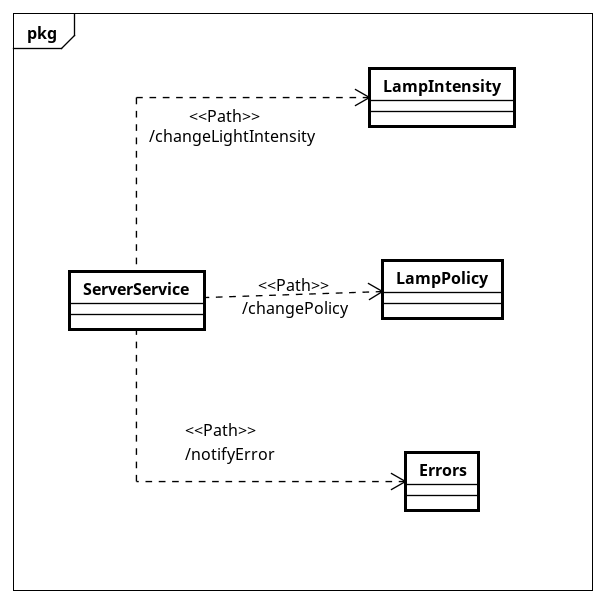
\includegraphics[scale=.8]{figure/Class_Diagram_Server_REST.png}
	\caption{API REST Servlet \label{API REST SERVLET}}
\end{figure}
\paragraph{Diagramma di sequenza}
In figura \ref{SEQ RPI TO SERVER} sono mostrate le interazioni tra Raspberry e servlet, e tra servlet e TS-DBMS.
\begin{figure}[tbp]
	\centering
	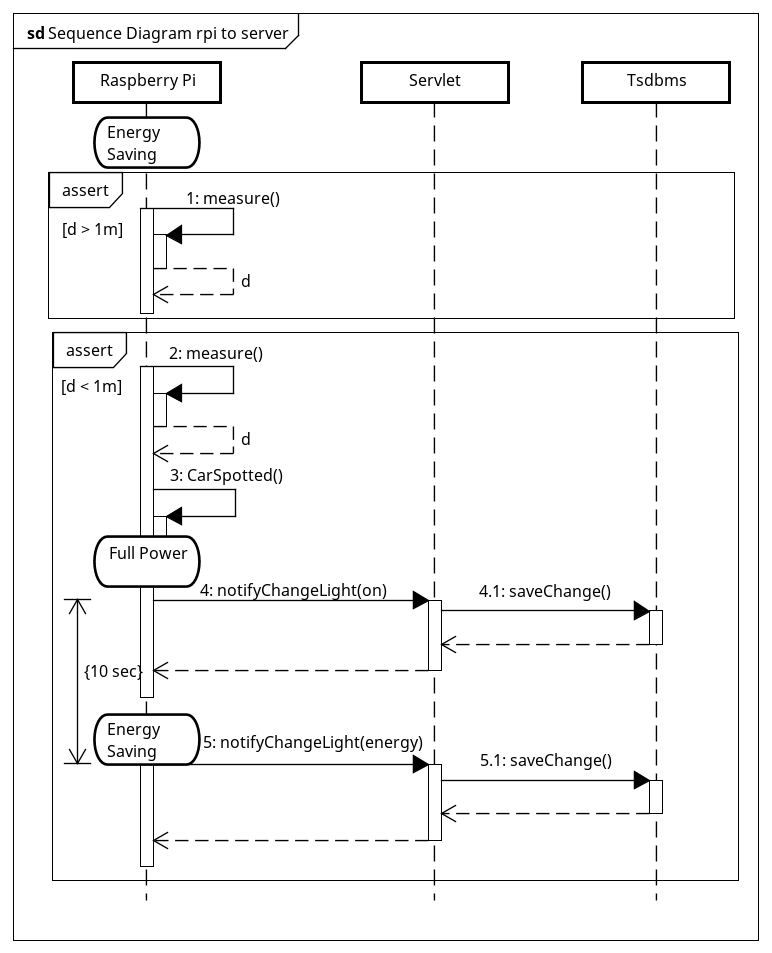
\includegraphics[scale=.65]{figure/Sequence_Diagram_rpi_to_server.png}
	\caption{Diagramma di sequenza delle comunicazioni tra Raspberry, servlet e TS-DBMS \label{SEQ RPI TO SERVER}}
\end{figure}

\newpage
\subsection{Sistema di generazione di statistiche e grafici}
La consultazione diretta dei dati memorizzati nel TS-DBMS può non essere user-friendly, e sicuramente non praticabile dall'utente medio.
Vale la pena quindi di garantire una modalità di fruizione maggiormente accessibile.
In particolare, si vuole rendere possibile la generazione di statistiche e grafici basati sui dati contenuti nel TS-DBMS.
Il sistema dovrà essere estendibile, in modo che i grafici non siano cablati all'interno del software, ma l'utente abbia modo di costruirli personalizzandoli in base alle proprie esigenze.
Una volta che tali grafici saranno costruiti, saranno fruibili anche dall'utente medio; l'utente avanzato sarà in grado di generare dinamicamente i grafici di cui ha bisogno.

\subsection{DBMS relazionale}
In aggiunta al TS-DBMS, si può valutare anche l'utilizzo di un DBMS relazionale per mantenere alcune informazioni semi-statiche o generate in quantità di gran lunga inferiori rispetto a quelle memorizzate nel TS-DBMS, quali:
\begin{itemize}
 \item l'anagrafica dei Raspberry dislocati sul territorio;
 \item le credenziali di accesso ai singoli Raspberry;
 \item eventuali dati statistici sintetici relativi allo storico dei guasti.
\end{itemize}


\section{Progettazione Raspberry}
Il sistema Raspberry fornisce le seguenti funzionalità:
\begin{itemize}
 \item rilevamento illuminazione ambientale con il sensore di luce;
 \item rilevamento presenza di automobili con i sensori di prossimità;
 \item illuminazione di ogni singolo lampione in base alle politiche locali;
 \item programma principale che gestisce il web server REST e l'invio delle statistiche al server.
\end{itemize}

\subsection{Architettura complessiva}
%TODO Parlare del paradigma ad attori
%TODO class diagram Raspberry Pi?

\subsection{Raspberry Pi architettura REST}
%TODO da ricontrollare e espandere?
I Raspberry devono offrire un'interfaccia REST che permetta di:
\begin{itemize}
	\item ottenere la configurazione attuale di un determinato lampione;
	\item modificare le policy di accensione e spegnimento;
	\item modificare le configurazioni per il risparmio energetico;
	\item permettere di iniziare a concludere una fase di debug per poter fare prove sul funzionamento dei lampioni;
	\item comunicare ai Raspberry vicini il sopraggiungere di un mezzo sulla carreggiata (comportamento locale ai Raspberry)
\end{itemize}

\subsection{Policy del sistema}
L'eventuale illuminazione di un lampione è regolata da policy stabilite in maniera centralizzata e modificabili anche mentre il sistema è in esecuzione.
A meno che non venga rilevato il passaggio di un'auto o di un livello di intensità luminosa eccedente il limite impostato nelle policy, l'unico fattore che viene considerato per l'accensione dei lampioni è l'orario corrente.
\paragraph{Macchina a stati finiti}
Per mostrare il comportamento del sistema riguardante le policy temporali si è utilizzata la macchina a stati finiti semplificata in figura \ref{FSM POLICY}.
Inizialmente i lampioni partono dallo stato \textit{off} e, se l'orario corrente (rappresentato dalla variabile \textit{t}) è successivo all'orario impostato per la policy \textit{on}, allora il lampione passerà allo stato \textit{on}.
In seguito, quando l'orario supererà la soglia di \textit{policy energy on}, il lampione andrà in modalità risparmio energetico passando allo stato \textit{energy saving}.
In tale modalità l'intensità luminosa sarà ridotta fino a quando non viene rilevato un mezzo in transito sulla carreggiata.
Alla fine del periodo di risparmio energetico, impostato da \textit{policy energy off}, il lampione tornerà allo stato di partenza, spegnendosi.
\begin{figure}[ht]
	\centering
	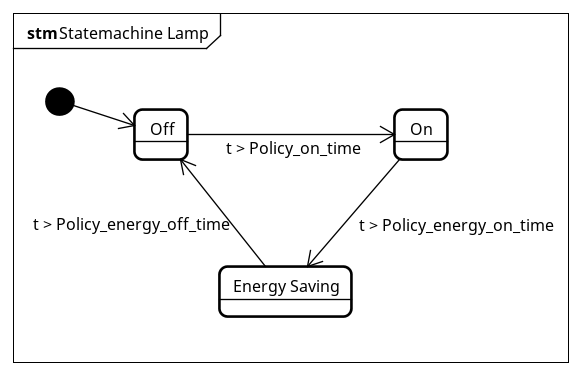
\includegraphics[scale=.8]{figure/Statemachine_Lamp.png}
	\caption{Finished State Machine relativo alle policy del sistema \label{FSM POLICY}}
\end{figure}

\newpage
\subsection{Controllo presenza auto}
Questa parte si occupa di controllare la presenza di eventuali mezzi in transito.
Utilizzando un sensore di prossimità, periodicamente viene calcolata la distanza tra il sensore e l'ostacolo più vicino per valutare se un'auto possa essere in transito in quel momento sulla carreggiata.
\paragraph{Comportamento sensore di prossimità}
Per la rappresentazione dell'architettura è stato scelto di utilizzare una ``Finished State Machine''.
Come si può notare in figura \ref{FSM CAR}, all'avvio di \textit{Ultrasonic} vengono avviati due comportamenti concorrenti: il primo ha il compito di aggiungere e rimuovere i lampioni interessati ad essere notificati del passaggio di auto; il secondo si occupa di fare la rilevazione della distanza tra il sensore e l'oggetto in quel momento più vicino.
Partendo dallo stato \textit{waiting}, se è presente almeno un attore, viene effettuata una lettura di distanza e, se il valore è maggiore della distanza tra il sensore e la larghezza della carreggiata, attende per qualche millisecondo e poi ritorna nello stato \textit{waiting}.
Se invece il valore è minore della larghezza della carreggiata, significa che è stato rilevato un mezzo in transito e quindi vengono notificati tutti i lampioni attualmente in lista.
Dopo aver aspettato qualche secondo, ritorna allo stato iniziale \textit{waiting}.
\begin{figure}[tbp]
	\centering
	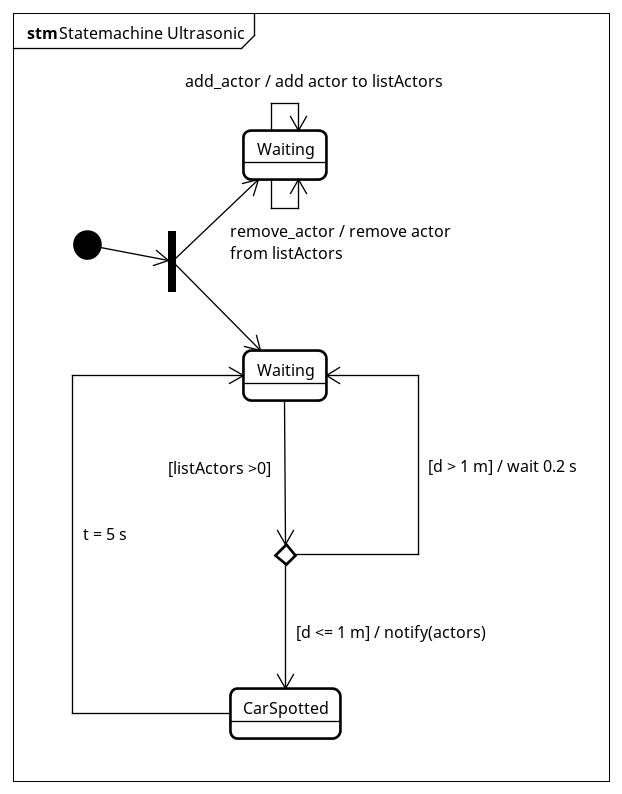
\includegraphics[scale=.75]{figure/Statemachine_Ultrasonic.png}
	\caption{Finished State Machine riguardante la parte di controllo presenza auto \label{FSM CAR}}
\end{figure}
\paragraph{Cambiamento di stato dei lampioni}
Utilizzando il diagramma di sequenza in figura \ref{SD CAR}, è stato rappresentato il cambio di stato da parte di due lampioni dal risparmio energetico alla piena potenza dopo la rilevazione di un'auto in transito.
Inizialmente i lampioni si trovano nello stato di risparmio energetico e viene effettuata una misurazione da parte del sensore di prossimità che restituisce la lettura rappresentata da \textit{d}.
Successivamente viene eseguita una seconda lettura: questa volta la distanza rilevata si assume equivalga a meno della soglia impostata come necessaria, e quindi che sia stata rilevata un'automobile.
Per questo vengono notificati entrambi i lampioni, i quali, dopo un intervallo di tempo calcolato tramite la moltiplicazione tra una costante e il proprio identificativo, passano in modalità di piena potenza per permettere all'automobilista di percorrere la strada in sicurezza.
\begin{figure}[tbp]
	\centering
	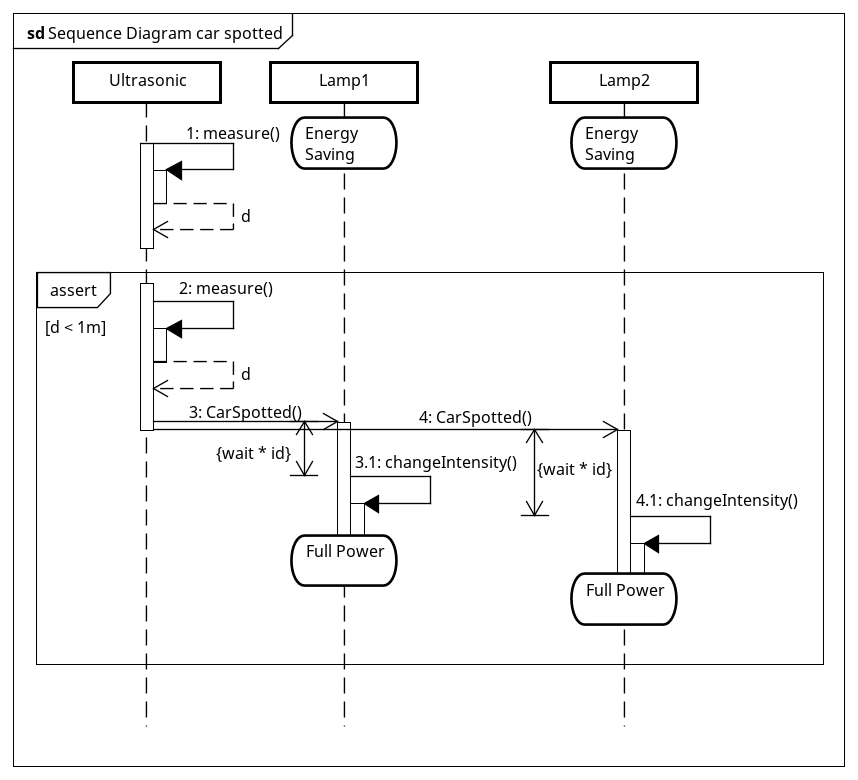
\includegraphics[scale=.59]{figure/Sequence_Diagram_car_spotted.png}
	\caption{Comunicazione tra il sensore ad ultrasuoni e i lampioni rappresentata tramite un Sequence Diagram \label{SD CAR}}
\end{figure}
\paragraph{Notifica ai dispositivi vicini}
Quando viene rilevato un mezzo in transito sulla carreggiata e tutti i lampioni di un determinato Raspberry si sono accesi, verrà comunicato ai dispositivi embedded successivi al proprio che un mezzo sta per sopraggiungere.
Come scritto in precedenza, le notifiche saranno messaggi di tipo REST.
Notificare i vicini è necessario per due motivi:
\begin{itemize}
	\item i lampioni successivi si potranno accendere tempestivamente;
	\item nel caso si giungesse ad un incrocio, verranno notificati tutti i dispositivi embedded relativi alle strade dell'intersezione.
\end{itemize}

\subsection{Controllo luminosità ambientale}
Questa parte si occupa di controllare l'intensità luminosa ambientale e di notificare i lampioni in modo che possano accendersi o spegnersi se il valore di luminosità fosse maggiore o minore di una certa soglia impostata nelle loro policy.
\paragraph{Architettura}
Per la rappresentazione dell'architettura è stato scelto di utilizzare una Finished State Machine.
In figura \ref{FSM PR} viene mostrato come inizialmente siano presenti due comportamenti concorrenti.
Come per il caso del controllo della presenza di auto, anche qui il primo è responsabile della gestione della lista dei lampioni da notificare;
il secondo si occupa di eseguire la lettura dell'intensità luminosa e di notificare ogni lampione presente nella lista.
\\Il secondo parte dallo stato \textit{waiting} ed esegue una lettura se la lista dei lampioni non è vuota.
In seguito invia la lettura effettuata a tutti gli elementi della lista e aspetta nello stato \textit{prMeasured} per qualche secondo.
Infine torna nello stato \textit{waiting}.
\begin{figure}[tbp]
	\centering
	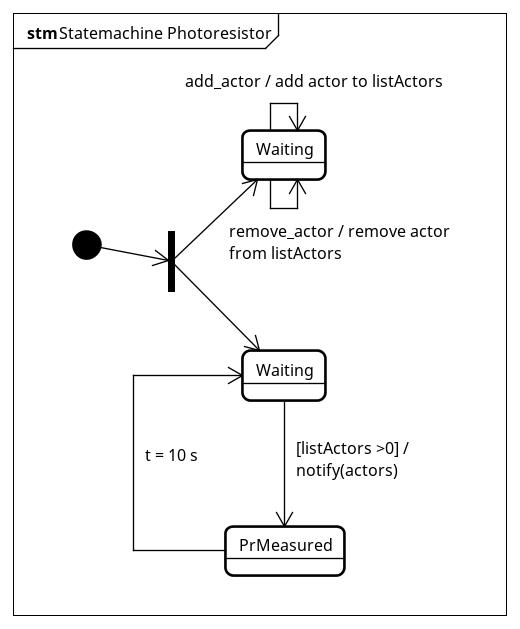
\includegraphics[scale=.8]{figure/Statemachine_Photoresistor.png}
	\caption{Finished State Machine riguardante la lettura della luminosità ambientale \label{FSM PR}}
\end{figure}

\newpage
\subsection{Web Server}
Il web server deve poter comunicare con i Raspberry dislocati sul territorio per poter ottenere e modificare le impostazioni locali di ogni dispositivo.
Per questo si mette in comunicazione con i Raspberry utilizzando le loro interfacce REST.
\paragraph{Diagramma di sequenza \label{seq-diagram-webserver}}
Come si può vedere in figura \ref{SD WEB} per la rappresentazione della comunicazione tra il web server e i Raspberry è stato utilizzato un diagramma di sequenza.
Nel primo esempio viene mostrata la richiesta da parte di un utente per ricevere le policy relative al lampione numero 1 da un determinato Raspberry.
Il web server utilizzando un URL prestabilito effettua una GET.
Il Raspberry ottiene le policy in formato JSON dal lampione 1 e restituisce tali informazioni al web server, che successivamente le mostrerà all'utente.
\\Il secondo esempio è simile al primo, con la differenza che in questo caso l'utente intende effettuare una modifica alla policy on del lampione 1.
Quindi il web server questa volta invierà una POST al Raspberry di competenza, il quale notificherà del cambiamento il lampione coinvolto.
Infine, verrà mostrato all'utente l'esito di tale operazione.
\begin{figure}[tbp]
	\centering
	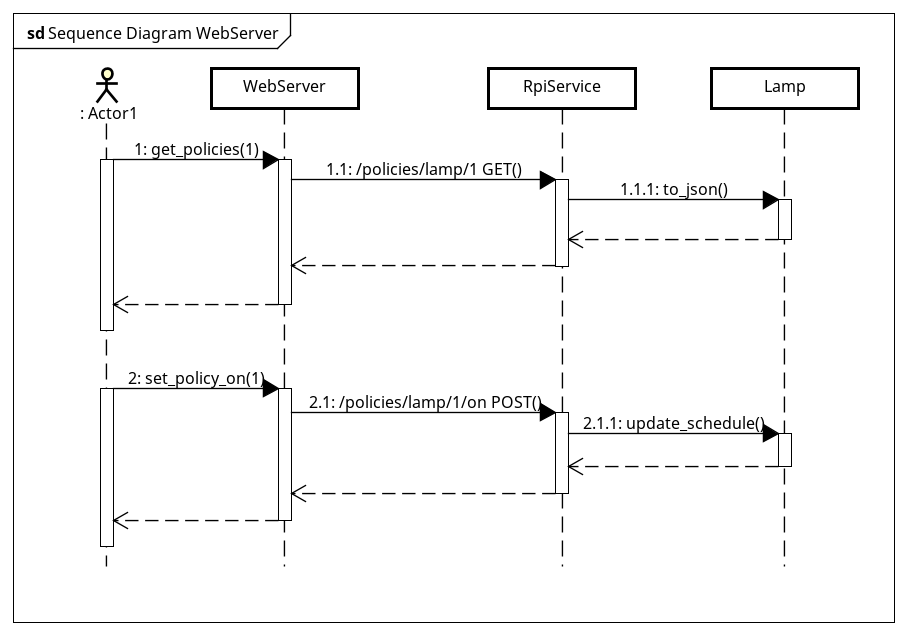
\includegraphics[scale=.55]{figure/Sequence_Diagram_WebServer.png}
	\caption{Sequence diagram per la comunicazione tra web server e Raspberry Pi \label{SD WEB}}
\end{figure}


\newpage
\section{Deployment}
Essendo i vari dispositivi Raspberry necessariamente dislocati sul territorio, si può agire su di essi solo variando il numero di lampioni controllati da ognuno.
Per quanto riguarda il lato server, invece, è possibile disaccoppiare i servizi su più server, al fine di migliorare le prestazioni e la ridondanza.
Verranno ora descritti i principali metodi di deployment.
Sono naturalmente possibili soluzioni intermedie.

\subsection{Centralizzazione totale}
Una soluzione è quella di installare tutti i servizi su un unico server (figura \ref{DD CENT}).
Questo minimizza i costi di deployment, ma limita le prestazioni e porta alla costituzione di un pericoloso ``single point of failure''.
La riduzione delle prestazioni può non essere un problema nel caso di sistemi di dimensioni ridotte, mentre lo è su sistemi più estesi.
La costituzione di un ``single point of failure'', invece, è da tenere bene in considerazione, in quanto un guasto sul server potrebbe causare problemi a tutto il sistema.
\begin{figure}[tbp]
	\centering
	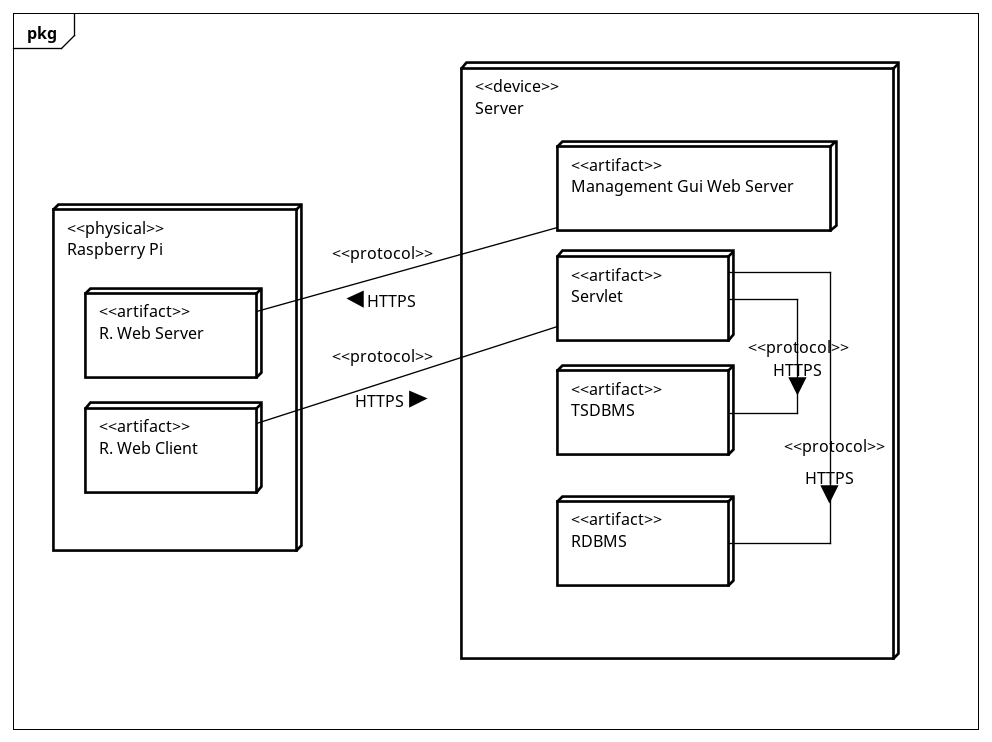
\includegraphics[scale=.5]{figure/Deployment_Diagram_2.png}
	\caption{Diagramma di deployment (server centralizzato) \label{DD CENT}}
\end{figure}

\subsection{Distribuzione}
La soluzione più scalabile e consigliata è quella di installare i vari servizi su server separati (figura \ref{DD DIST}): questo porta ad un forte incremento delle prestazioni, e riduce l'impatto derivante da eventuali guasti.
\begin{figure}[tbp]
	\centering
	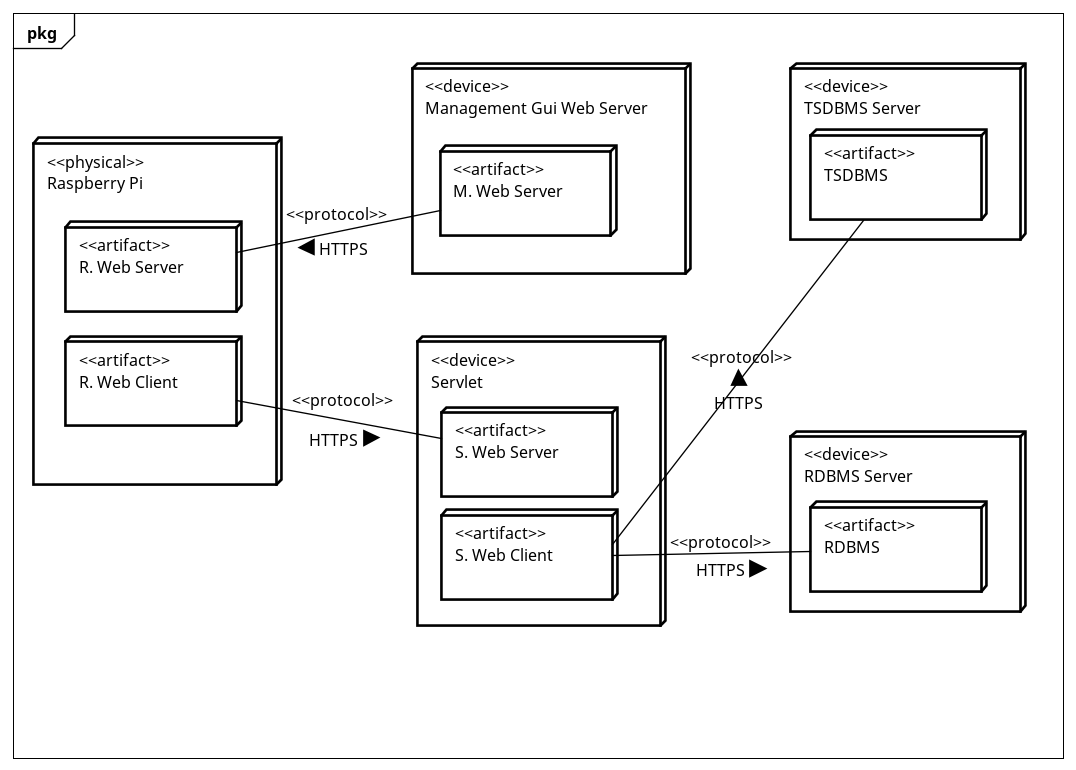
\includegraphics[scale=.45]{figure/Deployment_Diagram_1.png}
	\caption{Diagramma di deployment (server distribuito) \label{DD DIST}}
\end{figure}

\subsection{Layer di smistamento}
Un'ulteriore soluzione prevede di utilizzare un layer di smistamento, installando più istanze della servlet su server diversi (figura \ref{DD LAYERED}).
In questo modo il nucleo del traffico non convergerebbe direttamente sul server centrale, ma verrebbe smistato precedentemente, facendo attività di load balancing.
Inoltre, in caso di problemi con un'istanza specifica della servlet, solo i Raspberry direttamente collegati ad essa ne risentirebbero.
\begin{figure}[tbp]
	\centering
	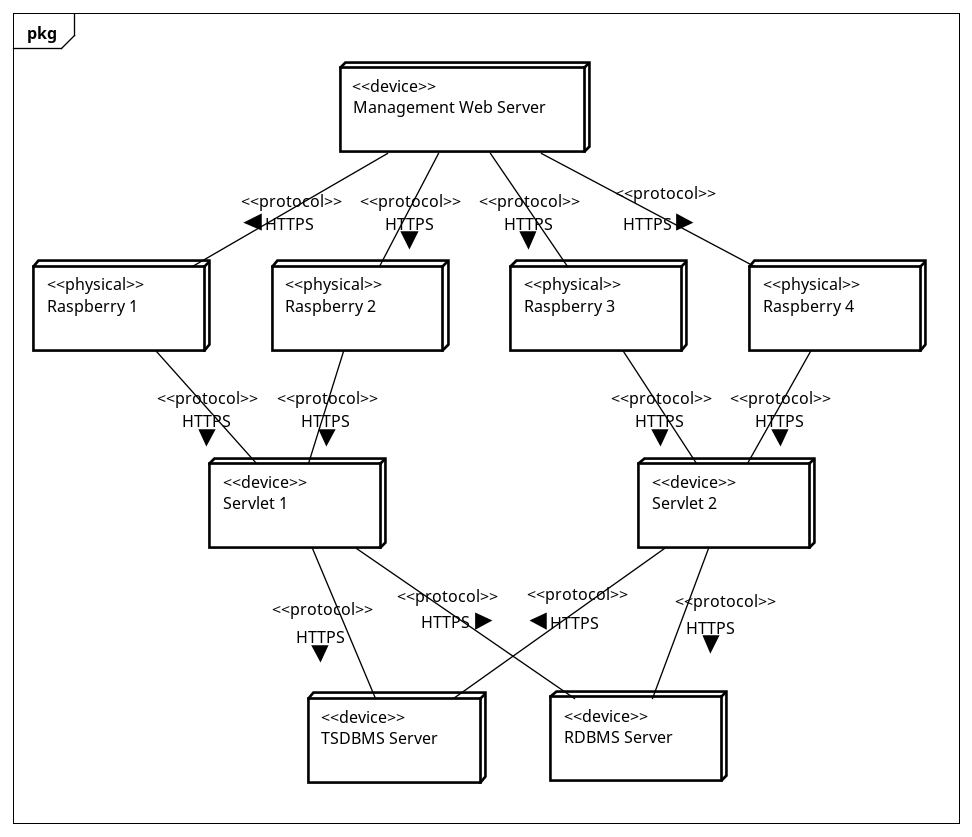
\includegraphics[scale=.45]{figure/Deployment_Diagram3v2.png}
	\caption{Diagramma di deployment (server distribuito) \label{DD LAYERED}}
\end{figure}


\section{Sicurezza}
Come evidenziato in fase di analisi dei requisiti, la sicurezza è un fattore critico per il successo del sistema.
Si rende quindi essenziale considerare la sicurezza già in fase di progettazione, in modo da minimizzare il numero e l'impatto delle eventuali vulnerabilità residue.
Per raggiungere questo scopo si agisce principalmente su due fronti: le comunicazioni di rete e il funzionamento interno dei servizi.

\subsection{Comunicazioni di rete}
Il primo aspetto di criticità è la modalità con cui avvengono le comunicazioni di rete, che costituiscono il fulcro del sistema.
Essendo il sistema pensato per funzionare sfruttando la rete Internet, occorre adottare opportune strategie per garantire autenticazione, riservatezza e integrità per ogni trasferimento dati.
Sono possibili anche varianti non basate su Internet, bensì su reti di tipologia differente.
La rete del sistema è suddivisibile in due macro-parti con caratteristiche diverse:
\begin{itemize}
 \item tra i Raspberry e la/le Servlet, caratterizzata da un elevata cardinalità e un ridotto traffico per singola connessione;
 \item tra la/le Servlet e il database, caratterizzata da un elevato volume di traffico su un singolo collegamento (o al limite poco più).
\end{itemize}
\paragraph{TLS}
Poiché le comunicazioni avvengono per design sfruttando interfacce REST e quindi il protocollo HTTP su TCP/IP, una prima possibilità è quella di adottare il protocollo TLS 1.2, la più recente versione di \textit{Transport Layer Security} (in futuro sarà possibile utilizzare le nuove versioni del protocollo con un aggiornamento software), che fornisce i servizi richiesti ed è lo standard del settore.
Ogni servizio sarà configurato in modo da accettare richieste solo con questo protocollo.
I dettagli sugli algoritmi crittografici e di hashing da utilizzare sono demandati all'implementazione, con la raccomandazione di consentire esclusivamente algoritmi sicuri e di disabilitare completamente quelli obsoleti.
Questa è la scelta che è stata effettuata per il sistema.
\paragraph{Rete ad hoc}
Una prima variante è quella di utilizzare una rete ad hoc separata da Internet.
Questa opzione, sebbene possibile, sarebbe probabilmente inutilmente costosa, in quanto richiederebbe la realizzazione di una nuova rete, senza possibilità di riutilizzare quella esistente.
Inoltre, la maggiore sicurezza derivante da questa architettura di rete appare ridondante, in quanto il protocollo TLS è sufficientemente sicuro da viaggiare su Internet senza rischi significativi.
Questa via potrebbe essere utile nel caso si scegliesse di utilizzare dispositivi embedded a capacità computazionale estremamente ridotta, al punto da non essere in grado di eseguire i calcoli crittografici necessari a TLS, oppure nel caso il sistema (o parte di esso) fosse fisicamente collocato in zone isolate, dove non è stata portata connettività Internet cablata, oppure nel caso la città già disponga di una propria rete utilizzata per altri scopi (ad esempio telecamere di videosorveglianza).
\paragraph{VPN}
Come alternativa alla crittografia basata su TLS, si può valutare di trasmettere i dati all'interno di tunnel VPN.
Questa opzione potrebbe essere scelta per evitare l'implementazione della crittografia come parte di questo sistema, appoggiandosi ad un servizio di sistema (la VPN) già sviluppato da terzi.
Tuttavia, questa scelta richiederebbe un tunnel VPN per ogni Raspberry (o piccolo gruppo di Raspberry), con conseguente aumento del carico sulle servlet, quindi appare poco sensata per il collegamento dei Raspberry alla Servlet, mentre potrebbe essere più ragionevole per quello tra Servlet e database.

\subsection{Sicurezza dei servizi}
I vari componenti software saranno scritti utilizzando linguaggi di alto livello che prevengano vulnerabilità di tipo buffer overflow.
In questo modo il problema viene spostato sugli interpreti o le macchine virtuali che eseguono il codice (ad esempio la \textit{Java Virtual Machine} (JVM) nel caso di Java).
L'accesso ai servizi dovrà essere ristretto tramite oppurtune policy dei firewall, in modo da esporre solo i servizi strettamente indispensabili, restringendoli, dove possibile, anche in base agli indirizzi IP (ad esempio, il TS-DBMS dovrà essere accessibile solo dalla/e servlet, e non dai Raspberry o da Internet in generale).
\paragraph{Virtualizzazione}
La modalità di deployment distribuita precedentemente descritta contribuisce ad un maggiore isolamento dei servizi rispetto alla modalità centralizzata.
Utilizzando macchine virtuali single-purpose è possibile mitigare notevolmente l'impatto di un'eventuale intrusione, dal momento che la compromissione di un server non implicherebbe quella totale di tutto il sistema.
In questo modo i tempi di risposta e ripristino da parte dei sistemisti sarebbe ridotto.
\paragraph{Permessi di esecuzione e MAC}
I servizi devono poter funzionare, dove possibile, con privilegi di esecuzione ridotti (idealmente, mai con i privilegi di root).
In questo modo, la compromissione di un servizio non comporterebbe automaticamente un danno per tutto il sistema.
Come ulteriore opzione, è possibile implementare sul sistema politiche di \textit{Mandatory Access Control} (MAC), in modo da confinare ulteriormente i servizi ai soli permessi strettamente necessari alla loro esecuzione.
Questo non vale solo per i servizi realizzati nell'ambito di questo progetto, ma anche per quelli installati sul sistema operativo, necessari al suo funzionamento.

\chapter{Implementazione}

In questo capitolo verranno descritte le scelte implementative, derivate dalle scelte progettuali.

\section{Implementazione della parte server - Sistemistica}
In questa sezione verrà illustrata la configurazione software del server e dei suoi servizi.

\subsection{Server}
Per una maggiore chiarezza nell'esposizione, verrà considerato uno schema di deployment con un unico server sul quale sono in esecuzione tutti i servizi.
Nel caso di server multipli, quanto detto in seguito vale allo stesso modo: l'unica differenza saranno gli indirizzi IP diversi per ogni server.
Tutto il software utilizzato e sviluppato è pensato per funzionare correttamente sia in un ambiente distribuito che centralizzato.
Nell'ambito dello sviluppo di questo progetto, si è utilizzato un server virtuale fornito dal provider DigitalOcean con la seguente configurazione hardware:
\begin{itemize}
 \item 512 MB di RAM;
 \item 1 vCPU;
 \item 20 GB di memoria secondaria su SSD;
 \item 1 TB di traffico di rete massimo mensile.
\end{itemize}
Una configurazione di questo tipo, seppure minimale, è più che adatta allo sviluppo e a piccole installazioni; per gestire sistemi di più grandi dimensioni si suggerisce una dotazione hardware più performante.
Ad ogni modo, come evidenziato in fase di progettazione, nel caso di installazioni di grandi dimensioni, si sconsiglia l'utilizzo di un unico server ad alte performance in favore di un cluster di più server individualmente meno potenti, al fine di garantire ridondanza.

\subsection{Sistema operativo, impostazioni e servizi di sistema}
Valutati i sistemi operativi presenti sul mercato, si è scelto di utilizzare una distribuzione Linux per i seguenti motivi:
\begin{itemize}
 \item coerenza con gli altri componenti del sistema;
 \item sistema operativo open source, quindi tendenzialmente più sicuro;
 \item possibilità di evitare costi di licenza, grazie alla licenza GNU-GPL.
\end{itemize}
In particolare, è stata utilizzata la distribuzione Ubuntu Server 16.04, basata sul kernel Linux 4.4, in quanto è una delle distribuzioni maggiormente diffuse in ambito server, è ben documentata, e utilizza software mediamente più aggiornato rispetto ad altre distribuzioni come Debian o CentOS.
Il software utilizzato è comunque disponibile per tutte le principali distribuzioni, quindi la scelta è in realtà libera, in base alle necessità delle singole installazioni.
Per motivi di sicurezza, è fondamentale aggiornare regolarmente i software installati per far fronte alle nuove vulnerabilità.
Questa operazione può essere eseguita manualmente da un sistemista, oppure pianificata automaticamente (nel caso di Ubuntu, configurando il pacchetto \textit{unattended-upgrades}).
\\Le seguenti funzionalità e servizi di sistema sono stati installati e configurati.
\paragraph{Utenti}
Per motivi di sicurezza è opportuno creare per ogni amministratore del server un utente distinto con privilegi ridotti.
Le operazioni che richiedono privilegi elevati devono essere eseguite utilizzando il comando \textit{sudo}, e mai autenticandosi direttamente come \textit{root}.
Ogni servizio in esecuzione dovrebbe idealmente essere eseguito utilizzando un account utente ad hoc dotato dei soli privilegi necessari all'esecuzione di quello specifico servizio.
\paragraph{AppArmor}
Come misura di sicurezza aggiuntiva, per limitare gli eventuali danni nel caso si verificasse un'intrusione, in aggiunta al Discretionary Access Control utilizzato da Linux, è buona norma utilizzare un meccanismo di Mandatory Access Control per confinare quanto più possibile ogni singolo processo.
Nell'ambito di questa installazione è stato utilizzato AppArmor. In alternativa, è possibile utilizzare SELinux, che fornisce un livello di granularità maggiore, ma è anche notevolmente più complesso da configurare.
Data la natura del servizio, tale per cui solo un amministratore è in grado di aprire una shell sul server, e non essendo i dati trattati critici, AppArmor è più che adeguato allo scopo.
\paragraph{SSH}
Il servizio SSH (Secure Shell) è utilizzato esclusivamente dall'amministratore per eseguire operazioni di manutenzione sul server.
Rispetto alla configurazione di default, sono state aggiunte alcune impostazioni di hardening, in quanto si tratta del servizio più appetibile per un eventuale attaccante: una compromissione di SSH consentirebbe di eseguire comandi dannosi, e aprirebbe la porta allo sfruttamento di vulnerabilità che potrebbero portare ad una privilege escalation a root, compromettendo l'intero server.
Le impostazioni aggiuntive di OpenSSH server sono:
\begin{itemize}
 \item consentire solo la versione 2 del protocollo SSH (la 1 è insicura);
 \item abilitazione dei soli algorigmi crittografici di scambio chiavi considerati robusti (\textit{curve25519-sha256@libssh.org,diffie-hellman-group-exchange-sha256}), disabilitando quelli meno sicuri (presenti per retrocompatibilità);
 \item disabilitazione dei moduli per lo scambio chiavi Diffie-Hellman con chiave più corta di 2048 bit;
 \item utilizzare chiavi private per il server di adeguata lunghezza e solo con algoritmi sicuri (\textit{ed25519,rsa});
 \item impedire l'autenticazione dei client tramite password, ma solo tramite chiavi asimmetriche (\textit{PasswordAuthentication no; ChallengeResponseAuthentication no; PubkeyAuthentication yes});
 \item abilitazione dei soli algoritmi di crittografia simmetrica considerati robusti (\textit{chacha20-poly1305@openssh.com,aes256-gcm@openssh.com,aes128-gcm@openssh.com,aes256-ctr,aes192-ctr,aes128-ctr}), disabilitando quelli meno sicuri (presenti per retrocompatibilità);
 \item abilitazione dei soli algorigmi MAC (Message Authentication Code) considerati robusti (\textit{hmac-sha2-512-etm@openssh.com,hmac-sha2-256-etm@openssh.com,hmac-ripemd160-etm@openssh.com,umac-128-etm@openssh.com,hmac-sha2-512,hmac-sha2-256,hmac-ripemd160,umac-128@openssh.com}), disabilitando quelli meno sicuri (presenti per retrocompatibilità);
 \item nel caso lo si ritenesse opportuno, è possibile implementare una forma di autenticazione a due fattori sfruttando un modulo PAM (Pluggable Authentication Module).
\end{itemize}
\paragraph{Fail2Ban}
Al fine di prevenire attacchi di tipo brute-force o basati su dizionario, può essere opportuno utilizzare \textit{Fail2Ban}, un demone che controlla nei file di log la presenza di tentativi di accesso non riusciti e di bloccare temporaneamente gli indirizzi IP dai quali provengono.
Per evitare che anche gli utenti legittimi vengano bloccati accidentalmente, è buona norma consentire un certo numero di tentativi prima di attuare il blocco.
Qualora l'indirizzo IP di un utente legittimo venisse bloccato, per tentare nuovamente di accedere è necessario attendere la scadenza del blocco o di accedere direttamente alla console del server.
\paragraph{UFW}
Essendo il sistema in rete, è necessario configurare il firewall per limitare il traffico ai soli servizi necessari. In questa implementazione è stato utilizzato \textit{UFW}, ma è possibile utilizzare anche \textit{iptables}.
Innanzitutto devono essere bloccate tutte le connessioni in ingresso ad eccezione di quelle necessarie al funzionamento del servizio. Quali siano effettivamente necessarie dipende dall'architettura di deployment (server singolo o più server) e dall'eventuale utilizzo di VPN.
Nel caso più semplice (tutti i servizi su uno stesso server), è necessario esporre verso l'esterno solamente SSH, il server web per la gestione e il sistema di generazione di grafici e statistiche.
Nel caso tutta la rete dei Raspberry fosse contenuta in una VPN o in una rete locale, si potrebbe esporre i singoli servizi solo sulle interfacce deputate a fornire quello specifico servizio.
In generale, il livello di isolamento sarà direttamente proporzionale alla sicurezza della rete.
Tuttavia, essendo tutte le informazioni in transito crittografate, il transito delle informazioni su rete pubblica non dovrebbe costituire un problema (salvo eventuali vulnerabilità scoperte in seguito nei software).
Anche nel caso il sistema trasmetta su una rete pubblica, qualora sia stata acquistata una sottorete di indirizzi IP pubblici, è consigliabile consentire connessioni solo da e verso gli indirizzi di quella sottorete.

\subsection{Server Web}
Il server web utilizzato per ospitare l'interfaccia di gestione dei Raspberry è \textit{nginx}. È stato scelto per:
\begin{itemize}
 \item la sua leggerezza;
 \item le elevate prestazioni;
 \item la scalabilità.
\end{itemize}
Allo stato attuale il carico su questo servizio si mantiene basso, in quanto le richieste che deve gestire sono poche contemporaneamente (solo gli operatori manutentori accedono a questo servizio).
Di conseguenza, è possibile utilizzare anche altri server web, ad esempio Apache. L'utilizzo di \textit{nginx} è stato pensato per far fronte ad eventuali nuove funzionalità future.
Come misura di sicurezza, tutte le connessioni sono protette tramite TLS 1.2, per evitare intercettazioni ed attacchi di tipo man-in-the-middle.
I dettagli implementativi dell'interfaccia web per controllare i Raspberry sono indicati in seguito nella sezione \ref{serv-rest-in}.

\subsection{Time Series DBMS \label{tsdbms}}
Come evidenziato in fase di progettazione, l'utilizzo di un Time Series database è particolarmente indicato per l'archiviazione dei dati statistici prodotti dai Raspberry.
Si è scelto di installare InfluxDB, un TS-DBMS open source sviluppato da InfluxData, scritto in \textit{Go} e ottimizzato per l'archiviazione di dati ad alte prestazioni, per la ricerca efficiente su serie di dati, e con supporto all'alta disponibilità.
La modalità principale di accesso ai dati è tramite un'interfaccia REST, in linea con i requisiti del sistema, sebbene esistano librerie per l'utilizzo con vari linguaggi di programmazione.
Nel caso di installazioni più piccole, sarebbe pensabile anche l'utilizzo di un DBMS relazionale, ma si rivelerebbe una scelta poco scalabile.
I dati vengono inviati ad InfluxDB esclusivamente dalle istanze della servlet, che fungono da mediatori tra i Raspberry e il database.
Sono stati implementati tre tipi di messaggi archiviabili sul database: \textit{changeLightIntensity}, \textit{changePolicy}, \textit{notifyError}.
\paragraph{Messaggio ``changeLightIntensity''}
Questo messaggio viene generato ogni qual volta un Raspberry modifichi l'intensità luminosa dei lampioni ad esso collegati e contiene i seguenti campi:
\begin{itemize}
 \item un riferimento all'host che ha generato l'evento;
 \item l'azione eseguita (accensione, spegnimento, variazione di luminosità dovuta a politiche di risparmio energetico o al passaggio di un'auto);
 \item un riferimento alla zona/gruppo in cui il Raspberry si trova;
 \item l'intensità luminosa impostata;
 \item l'intensità di luce ambientale rilevata;
 \item un timestamp relativo al momento della generazione dell'evento.
\end{itemize}
\paragraph{Messaggio ``changePolicy''}
Questo messaggio viene generato quando vengono modificate le policy di un lampione (orari di accensione e spegnimento e soglie di luminosità.
In questo caso vengono registrati i seguenti parametri:
\begin{itemize}
 \item un riferimento all'host che ha generato l'evento;
 \item un riferimento alla zona/gruppo in cui il Raspberry si trova;
 \item un timestamp relativo al momento della generazione dell'evento.
\end{itemize}
\paragraph{Messaggio ``notifyError''}
Questo messaggio viene generato quando un Raspberry auto-diagnostica un errore interno e ha lo scopo di avvisare l'amministratore che è necessario un intervento manuale.

\subsection{Sistema di generazione di statistiche e grafici}
Per analizzare in maniera proficua la grande quantità di dati potenzialmente archiviata del database InfluxDB si è scelto di utilizzare il software \textit{Grafana}, software specializzato nella generazione di grafici statistici basati sui dati contenuti in TS-DBMS.
La scelta è ricaduta su questo strumento specifico in quanto è estremamente flessibile, consentendo agli amministratori di generare i grafici di loro interesse filtrando e aggregando i dati.
In questo modo gli amministratori possono creare dinamicamente i grafici di cui hanno bisogno, adattandosi in questo modo sia alla topologia della città in cui il sistema è installato, sia alle necessità specigiche che potrebbero sorgere in maniera imprevedibile (ad esempio potrebbe sopraggiungere la necessità di monitorare con maggiore granularità un'area della città in particolare, qualora si rilevasse un numero di guasti fuori norma).
Gli amministratori potranno quindi creare alcuni grafici di interesse generale sempre disponibili e altri dinamicamente in base alle necessità, in maniera simile a quello che avviene nella navigazione di un data-warehouse, ma orientato alle serie di dati.
I grafici sono creabili e consultabili utilizzando l'interfaccia web di Grafana. Qualora si rendesse necessario creare grafici estremamente personalizzati, è anche possibile scrivere direttamente le query per interrogare il database.
Per il rilevamento di guasti, si possono generare grafici che mettono in risalto comportamenti al di fuori della media (lampioni che si accendono in orari completamente diversi dagli altri, Raspberry che improvvisamente smettono di inviare dati, ecc.).
% TODO inserire uno screen di grafana

\subsection{DBMS relazionale}
Opzionalmente, si può valutare di utilizzare un database relazionale di supporto per memorizzare:
\begin{itemize}
 \item l'anagrafica dei Raspberry dislocati sul territorio;
 \item le credenziali di accesso ai singoli Raspberry;
 \item eventuali dati statistici sintetici relativi allo storico dei guasti.
\end{itemize}
% TODO Da rivedere


\section{Implementazione della servlet \label{serv-impl}}
Come descritto nell'architettura nel capitolo precedente, i dispositivi Raspberry non comunicano direttamente con il database, ma si affidano ad una o più istanze di una servlet intermediaria.
Il linguaggio di programmazione scelto per l'implementazione è Java, poiché è disponibile per un'ampia varietà di sistemi operativi ed esiste un ampio supporto da parte di librerie esterne.
Data la natura dell'applicazione, che necessita di reattività e scalabilità, l'implementazione è stata realizzata sfruttando \textit{Vert.x}, una libreria integrabile in Java che consente di utilizzare un paradigma event-driven e non bloccante, particolarmente indicata per la realizzazione di microservizi REST.
Resta comunque possibile implementare la servlet con altre tecnologie e linguaggi di programmazione, a patto di mantenere invariate le interfacce REST.

\subsection{Interfaccia REST in ingresso \label{serv-rest-in}}
La servlet viene contattata dai Raspberry (client) con un messaggio JSON contenente una serie di dati, dipendente dal tipo di messaggio. Tutte le connessioni crittografate e autenticate con TLS.
I possibili campi sono:
\begin{itemize}
 \item "area": campo numerico che corrisponde alla zona di appartenenza del lampione. Serve a fini statistici per aggregare i dati;
 \item "action": campo che corrisponde al tipo di azione che è stata eseguita, e può essere uno tra: \textit{turn\_on}, \textit{turn\_off}, \textit{energy\_saving} o \textit{car\_detected};
 \item "intensity": campo numerico relativo all'intensità di luce attuale del lampione;
 \item "photoresistor": campo numerico relativo alla lettura della fotoresistenza;
 \item "timestamp": campo che contiene il timestamp in cui è avvenuta l'azione.
\end{itemize}

\subsection{Interfaccia REST in uscita}
La servlet, nel suo ruolo di mediatore, esegue la conversione dei dati JSON ricevuti dai Raspberry nel formato richiesto dal database, e lo contatta utilizzando a sua volta un'interfaccia REST (in questo caso la servlet si comporta da client rispetto al database (server)).
Il contenuto dei messaggi è descritto nella parte di dettaglio del Time Series Database (sezione \ref{serv-rest-in}).
Per motivi di sicurezza, ad ogni risposta ai client, vengono inseriti alcuni header HTTP per mitigare l'impatto di vulnerabilità Cross Site Scripting (XSS) e altri usi scorretti, oltre a disabilitare il caching (non necessario in questo tipo di applicazione).

\subsection{Parametri della servlet}
Se avviata senza specificare alcun parametro, la servlet utilizzerà quelli di default; è altrimenti possibile specificarli tramite argomenti dalla linea di comando. I parametri sono:
\begin{itemize}
 \item \textit{dbhost}: indirizzo IP del database (di default 127.0.0.1);
 \item \textit{listenPort}: porta TCP sulla quale la servlet è in ascolto (di default 44343);
 \item \textit{dbPort}: porta TCP sulla quale il TS-DBMS è in ascolto (di default 8086);
 \item \textit{dbName}: nome del database sul server TS-DBMS (di default ``esls'').
\end{itemize}
Altri parametri hard-coded sono:
\begin{itemize}
 \item \textit{API\_LEVEL}: numero di versione dell'interfaccia REST (inviato dai Raspberry ad ogni richiesta REST, utile per mantenere retrocompatiblità con eventuali nuove versioni della servlet e del software su Raspberry);
 \item \textit{BODY\_SIZE\_LIMIT}: limita la dimensione del buffer per le richieste HTTP in ingresso (utile per mitigare gli attacchi DDoS)
\end{itemize}


\section{Implementazione della parte embedded - Raspberry}
In questa sezione verrà illustrata l'implementazione della parte Raspberry.

\subsection{Hardware}
%TODO
\paragraph{Raspberry Pi}
%TODO dotazione hardware raspberry
\paragraph{Sensori e attuatori}
%TODO sensori e attuatori utilizzati

\subsection{Sistema operativo e servizi di sistema}
Per quanto riguarda la scelta del sistema operativo da utilizzare, la scelta è ricaduta sulla distribuzione Linux Raspbian, in quanto è la principale distribuzione ufficialmente supportata per Raspberry e, basandosi su Debian, offre un livelli di leggerezza, stabilità e sicurezza elevati.
Queste caratteristiche sono di grande importanza in un sistema di questo tipo, ovvero in cui i Raspberry sono dislocati sul territorio e collegati in rete.
Ad ogni modo, sebbene la scelta della distribuzione sia ricaduta su Raspbian, è possibile utilizzare una qualsiasi altra distribuzione Linux semplicemente installando tutte le dipendenze necessarie che verranno utilizzane in fase di implementazione del progetto.
\paragraph{Nota sulla gestione del tempo}
I messaggi che i Raspberry Pi inviano quando comunicano con il server contengono al loro interno anche un timestamp per fini statistici.
Per evitare che col passare del tempo l'orario vada fuori sincrono, si è impostato l'aggiornamento tramite server \textit{NTP} su base giornaliera invece che, come di default, ad ogni avvio: i Raspberry possono restare attivi per lunghi periodi senza essere riavviati.
\paragraph{SSH}
%TODO (vedere anche la mia sezione su ssh più in alto in questo capitolo per i concetti di base. Però più sintetica)

\subsection{Linguaggio di programmazione, paradigma ad attori e organizzazione a task}
Per il programma in esecuzione sui Raspberry Pi si è scelto di utilizzare Python 3, che garantisce un elevato supporto per i sensori e attuatori attualmente disponibili.
%TODO Aggiungere qualcosa per tessere le lodi di Python (perché proprio Python e non C/Java/qualunque altra cosa?)
Essendo il software dei Raspberry composto da diverse parti tra loro autonome e concorrenti, si è scelto di utilizzare il paradigma ad attori (tramite la libreria \textit{Pykka}), un modello computazione concorrente a più alto livello rispetto alla gestione manuale dei thread, in quanto si addice maggiormente alla struttura interna del progetto.
In questo modo ogni componente logica è un attore e la comunicazione avviene esclusivamente tramite scambio di messaggi. In risposta ad un messaggio ricevuto un attore può:
\begin{itemize}
 \item prendere una decisione locale;
 \item creare nuovi attori;
 \item inviare nuovi messaggi;
 \item determinare come rispondere al successivo messaggio che potrà ricevere.
\end{itemize}
Come definito in fase di progettazione, i Raspberry devono poter eseguire diverse operazioni concorrentemente, tra cui:
\begin{itemize}
 \item rimanere in ascolto per eventuali richieste REST;
 \item controllo della presenza di auto;
 \item rilevamento dell'intensità luminosa;
 \item gestione dell'illuminazione dei lampioni in base ad uno scheduling.
\end{itemize}
La libreria \textit{threading} di Python, che permette ad un singolo programma l'esecuzione di più thread, è stata impiegata.

\subsection{Controllo presenza auto \label{cpa}}
Per controllare la presenza di auto sulla carreggiata viene effettuato il calcolo della distanza utilizzando il sensore ad ultrasuoni HC-SR04.
Per mitigare eventuali errori grossolani vengono effettuate sempre due misurazioni, calcolando successivamente la media.
La misurazione avviene inviando un segnale ad ultrasuoni e calcolando il tempo che il segnale impiega per andare e tornare, rimbalzando sugli oggetti.
Per calcolare la distanza in centimetri si moltiplica il tempo per la velocità del suono nell'aria (34300 cm/s) e il tutto viene diviso per 2 (perché il tempo era relativo all'andata e ritorno).
Per capire la direzione di marcia di un auto, nel caso di strade a doppio senso di marcia, è possibile adottare due strategie.
\begin{itemize}
 \item Posizionare nelle vicinanze del primo e dell'ultimo lampione, controllati da un determinato Raspberry, una coppia di sensori ad ultrasuoni a qualche centimetro di distanza tra loro: in questo modo controllando in quale sequenza la coppia di sensori rileva la presenza di un auto è possibile intuirne la direzione di marcia.
 \item Posizionare in tutto due sensori ad ultrasuoni vicino ai lampioni controllati da un determinato Raspberry: il primo andrà posizionato vicino al primo lampione sullo stesso lato della strada, e il secondo andrà vicino all'ultimo lampione sul lato opposto della strada.
 In questo modo impostando una soglia per il rilevamento delle auto pari al limite delle due carreggiate sarà possibile valutare il senso di marcia delle auto.
 Quindi, se per esempio il limite della carreggiata si trova a due metri dal bordo della strada, si imposterà il sensore in modo che se rilevi solo oggetti distanti meno di due metri, ed essi verranno considerati auto in transito sulla propria carreggiata.
\end{itemize}
Per l'implementazione di questo progetto si è optato per l'utilizzo della seconda strategia perché consente di ottenere lo stesso risultato utilizzando solo due sensori ad ultrasuoni invece che quattro, contenendo i costi.
L'utilizzo della prima strategia potrebbe tornare utile nel caso si voglia calcolare anche la velocità di crociera dei veicoli in transito.
In questo progetto essere in grado di capire il senso di marcia permette di accendere i lampioni in sequenza seguendo il verso di percorrenza.
Il thread che si occupa del sensore di prossimità utilizza un secondo thread per inviare il segnale ad ultrasuoni.
Grazie a questa scelta si evita che il thread principale del sensore vada in busy waiting attendendo l'invio e il ritorno del segnale ad ultrasuoni.
Inoltre si è utilizzata la funzione \textit{wait\_for\_edge} che permette di fermare l'esecuzione del thread fino a quando non viene rilevata un'oscillazione, consumando una quantità minima di CPU.
Per impostazione predefinita, il processo di misurazione considera la presenza di un veicolo sulla strada se la distanza rilevata è minore di due metri.
Tale valore può essere facilmente regolato in base alle caratteristiche della strada in cui si intende installare i sensori.
Il processo di controllo presenza auto è rappresentato da un attore il quale, dopo aver effettuato un controllo, notifica tutti i lampioni interessati.

\newpage
\lstinputlisting{code/ultrasonic.py}

\subsection{Rilevamento intensità luminosa}
Considerando che il Raspberry Pi non dispone di PIN analogici, per effettuare le letture di luminosità è possibile utilizzare le seguenti modalità:
\begin{itemize}
 \item collegare un altro controllore che abbia pin analogici (ad esempio Arduino) e utilizzare una fotoresistenza analogica;
 \item utilizzare una fotoresistenza analogica collegandola ad un convertitore analogico-digitale (ADC);
 \item utilizzare un sensore di luminosità digitale.
\end{itemize}
La prima modalità potrebbe essere presa in considerazione nel caso in cui si debba utilizzare diversi tipi di sensori analogici, tali da giustificare l'utilizzo di un controllore esterno, che comporterebbe maggiori costi e introdurrebbe complessità nel sistema.
Anche la seconda modalità può essere utile se si deve utilizzare più di un sensore analogico visto che un singolo ADC permette di utilizzare diversi pin analogici, ma è conveniente rispetto alla prima, in quanto più economica e non introduce particolare complessità.
In questo caso, dovendo collegare una singola fotoresistenza, si è optato per la terza modalità, utilizzando il sensore digitale TSL2561.
In alternativa si potrebbe prevedere l'utilizzo di più sensori di luminosità in modo da essere in grado di effettuare una media delle letture, compensando eventuali letture errate dovute ad eventuali danneggiamenti o residui di sporco che potrebbero coprire il sensore.
Come per il controllo di presenza di auto della sezione \ref{cpa}, anche il processo di rilevamento è gestito da un attore.

\subsection{Scheduling illuminazione \label{si}}
%TODO questa sezione è lunga e poco strutturata. Valutare di spezzarla in più paragraph o, se complicasse troppo la formattazione, al limite di andare a capo quando si cambia argomento
Per quanto riguarda la programmazione dell'illuminazione, il sistema offre la possibilità di impostare su base giornaliera un orario di accensione, di spegnimento, di inizio e di fine del periodo di risparmio energetico.
% in fase di progettazione è stato spiegato cos'è il periodo di risparmio energetico?
In tutte e quattro le impostazioni, oltre all'orario, è previsto anche un campo relativo alla soglia di intensità luminosa desiderata.
Come scelta implementativa, si è deciso di dare la precedenza alla luminosità rilevata rispetto all'orario.
Di conseguenza il funzionamento sarà il seguente: supponiamo di aver programmato l'accensione dei lampioni per le 19:00 con un livello di luminosità nell'ambiente pari a 50.
Se alle 19:00 l'intensità luminosa rilevata fosse minore di 50, i lampioni si accenderebbero; nel caso in cui l'intensità luminosa fosse maggiore di 50 i lampioni rimarrebbero spenti nonostante siano le 19:00.
È stata effettuata questa scelta perché se la luminosità esterna rilevata fosse alta sarebbe poco sensato accendere anche i lampioni.
Al contrario, se la luminosità rilevata fosse bassa, questo potrebbe anche essere dovuto a residui di sporco che con il tempo potrebbero depositarsi sul sensore.
Quindi anche se si rileva un livello di luminosità basso, si aspetta comunque l'orario impostato per accendere i lampioni.
La programmazione temporale viene espressa con precisione al minuto, visto che considerare anche i secondi comporterebbe un livello di precisione inutilmente elevato per questo scenario applicativo.
La configurazione dei lampioni potrebbe essere salvata:
\begin{itemize}
 \item in locale su ogni dispositivo embedded o su un server centralizzato;
 \item utilizzando un database relazionale o un file di testo.
\end{itemize}
Salvando le configurazioni su un server centrale si avrebbe il vantaggio di poter effettuare query consultando un singolo server e di gestire facilmente il backup centralizzato delle configurazioni;
d'altro canto, ogni dispositivo embedded dovrebbe sempre contattare il server per poter venire a conoscenza della propria programmazione e, nel caso in cui la connessione ad internet venisse a mancare, il dispositivo embedded smetterebbe di funzionare.
Salvando le configurazioni in locale su ogni Raspberry si ha una maggiore resistenza ai guasti visto che, anche nel caso in cui la connessione internet venisse persa, il dispositivo embedded potrebbe continuare a funzionare essendo il proprio comportamento totalmente locale.
Un database relazionale potenzialmente potrebbe offrire prestazioni maggiori rispetto ad un file di testo, ma tale vantaggio sarebbe evidente solo nel caso in cui i dati da salvare fossero in numero considerevole, e non è questo il caso;
un file di testo con una certa sintassi permette di controllare i valori salvati e di modificarli anche manualmente agendo direttamente sul file senza effettuare complicate query SQL.
Considerando i requisiti di progettazione come l'affidabilità del sistema e la facilità di gestione, si è scelto di salvare le configurazioni utilizzando un file di testo locale su ogni dispositivo embedded.
Inoltre il deploy dei dispositivi embedded potrebbe essere automatizzato, ad esempio tramite l'utilizzo di software quali \textit{Ansible} o \textit{Puppet}.
Grazie a questa scelta gli addetti ai lavori possono effettuare una programmazione agevole su ogni singolo lampione sia tramite interfaccia web che direttamente modificando i file di testo (tramite SSH o localmente).
Per il formato con cui vengono salvate le configurazioni si è scelto di utilizzare il \textit{Configuration file parser} presente nelle librerie standard di Python, perché permette la creazione di configurazioni con un linguaggio semplice, con una struttura simile ai file \textit{INI} di Microsoft Windows.
Questo garantisce una facile lettura e modifica anche manuale dei file. I file così creati hanno una estensione \textit{cfg}. I file hanno quattro sezioni principali con diversi campi ciascuna.
La prima sezione è \textit{GENERAL} e prevede tre campi:
\begin{itemize}
 \item \textit{lamp\_id}: un identificativo intero progressivo del singolo lampione;
 \item \textit{lamp\_pin}: il numero del pin a cui il lampione è collegato sul dispositivo embedded;
 \item \textit{lamp\_area}: la zona di appartenenza del singolo lampione.
\end{itemize}
La seconda sezione \textit{LampPolicyOn} e la terza \textit{LampPolicyOff} hanno gli stessi campi:
\begin{itemize}
 \item \textit{intensity}: l'intensità di luce del lampione espressa con un numero da 0 a 100 (impostare l'intensità a 0 equivale a spegnere il lampione);
 \item \textit{time\_h}: l'ora a cui questa impostazione dovrà iniziare;
 \item \textit{time\_m}: il minuto a cui questa impostazione dovrà iniziare;
 \item \textit{photoresistor}: la soglia richiesta di luminosità ambientale.
\end{itemize}
La quarta sezione è \textit{LampEnergySaving} e prevede cinque campi:
\begin{itemize}
 \item \textit{intensity}: l'intensità di luce del lampione espressa con un numero da 0 a 100;
 \item \textit{time\_h\_on} e \textit{time\_m\_on}: rispettivamente l'ora e i minuti in cui inizia la modalità risparmio energetico;
 \item \textit{time\_h\_on} e \textit{time\_m\_on}: rispettivamente l'ora e i minuti in cui termina la modalità risparmio energetico.
\end{itemize}
Per una questione di coerenza l'inizio e la fine della modalità risparmio energetico deve essere obbligatoriamente compresa tra \textit{LampPolicyOn} e \textit{LampPolicyOff}.
In definitiva grazie a tale implementazione si è reso possibile sia la modifica dello scheduling di un singolo lampione con la comodità della interfaccia web, sia una modifica più avanzata collegandosi per esempio in SSH ad un Raspberry e cambiando i valori manualmente sui file di configurazione.

\lstinputlisting{code/light0.cfg}
\newpage

\subsection{Messaggi a fini statistici}
Quando i dispositivi embedded eseguono azioni rilevanti, inviano ad un'istanza della servlet (sezione \ref{serv-impl}) un messaggio \textit{JSON} per consentire agli addetti ai lavori di avere una panoramica generale sull'andamento dell'intero sistema.
I possibili campi del messaggio sono stati descritti nella sezione \ref{serv-rest-in} relativa all'implementazione della servlet.

\subsection{API REST}
Come scritto in fase di progettazione, i Raspberry Pi devono esporre un insieme di API di tipo REST per consentire la modifica delle policy relative alla programmazione dei lampioni.
Per tale scopo è stata utilizzata la libreria \textit{Flask}.
Quando un Raspberry riceve una richiesta tramite la API REST, per prima cosa vengono controllate le credenziali fornite, in quanto è sempre richiesta un'autenticazione tramite username e password per poter completare una qualsiasi operazione GET o POST.
Nel caso la richiesta ricevuta sia valida, verrà restituito un JSON contenente o i dati richiesti, o il codice di stato HTTP 200 (nel caso in cui la richiesta non preveda dati di ritorno) per confermare la riuscita dell'operazione.
%da rivedere e espandere

\subsection{Modalità Debug}
Per consentire agli addetti ai lavori di effettuare controlli sui lampioni, come per esempio verificare il loro corretto funzionamento, è stata prevista la possibilità di abilitare la modalità debug.
Entrando in modalità debug i lampioni si accenderanno e spegneranno in base ai comandi che verranno impartiti manualmente, ignorando le eventuali policy impostate in precedenza.
Per abilitarla è necessario inviare una richiesta POST all'indirizzo \textit{/debug/lamp/<int:lamp\_id>/on} (per accendere un lampione) oppure a \textit{/debug/lamp/<int:lamp\_id>/off} (per spegnere un lampione).
Le richieste POST dovranno contenere un campo \textit{intensity} che corrisponde all'intensità luminosa desiderata a cui si intende impostare il lampione.
Quando si vuole concludere la fase di debug bisogna inviare una POST all'indirizzo \textit{/debug/lamp/<int:lamp\_id>/stop}.
Una volta conclusa la fase di debug, i lampioni torneranno a funzionare seguendo il proprio scheduling.

\subsection{Gestione dei guasti}
%TODO: cosa succede se un rasp si rompe? Cosa continua a funzionare e cosa no a seconda del tipo di guasto (guasto di rete, hardware, ...). Parlare anche della notifica del guasto al server (ipotizzando di avere hardware che si accorge dei led bruciati, che però nella nostra implementazione non c'è, ma il software deve supportarlo).

\section{Implementazione dell'interfaccia Web di manutenzione}
Come illustrato nella sezione \ref{si}, per permettere agli addetti ai lavori di controllare e modificare la programmazione dei singoli lampioni è stata implementata un'interfaccia Web tramite un server REST.
Come misura di sicurezza, tutte le richieste GET e POST ai Raspberry dovranno essere corredate da nome utente e password relativi al singolo dispositivo embedded che si intende contattare.
%(mmm, la storia del "dare ad un addetto solo le credenziali dei rpi della sua zona dove lo mettiamo?) --> nella sezione DBMS relazionale. Ma al momento non è implementato, quindi aspetto a scriverlo.
Il sito Web è stato realizzato seguendo uno stile minimale, moderno e il quanto più intuitivo per l'utente.
L'interfaccia è ottimizzata sia per un uso desktop che mobile.
\begin{figure}[tbp]
	\centering
	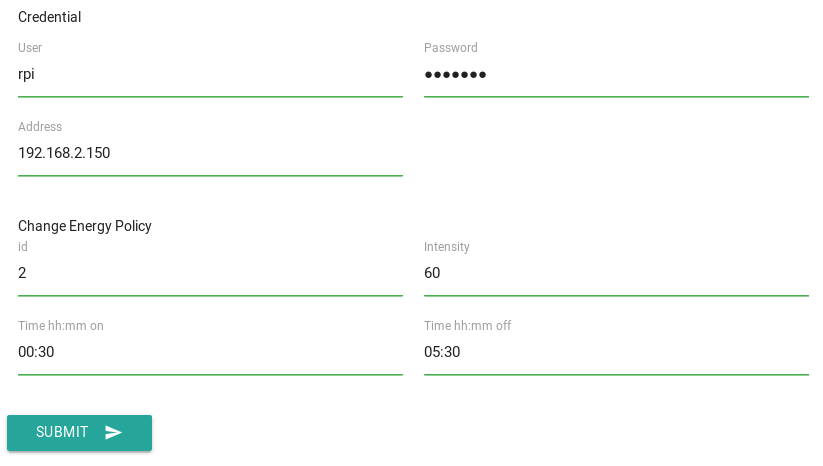
\includegraphics[scale=.62]{figure/web_desktop.png}
	\caption{Interfaccia web Desktop \label{WD}}
	\subfloat[(Mobile) Campi corretti]{{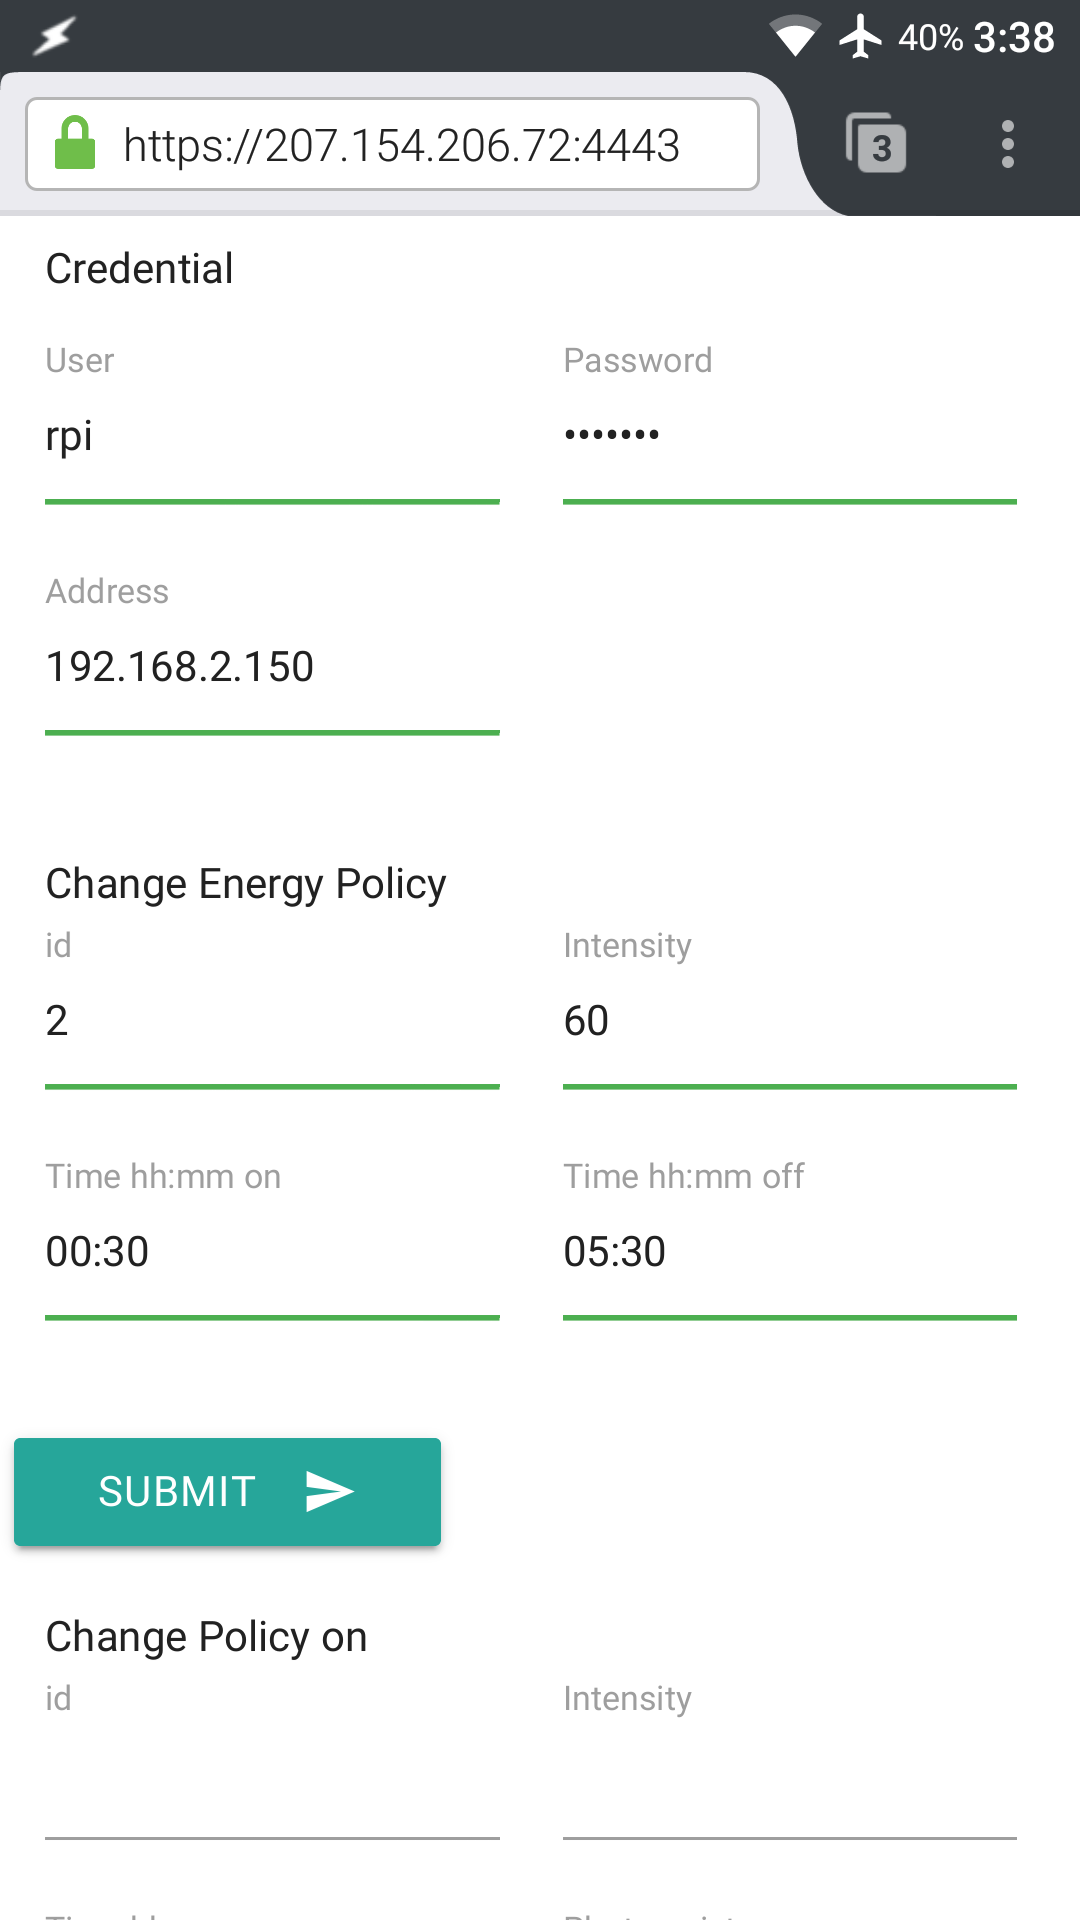
\includegraphics[width=6cm]{figure/web_mobile.png} }}%
	\qquad
	\subfloat[(Mobile) Campi mancanti o errati]{{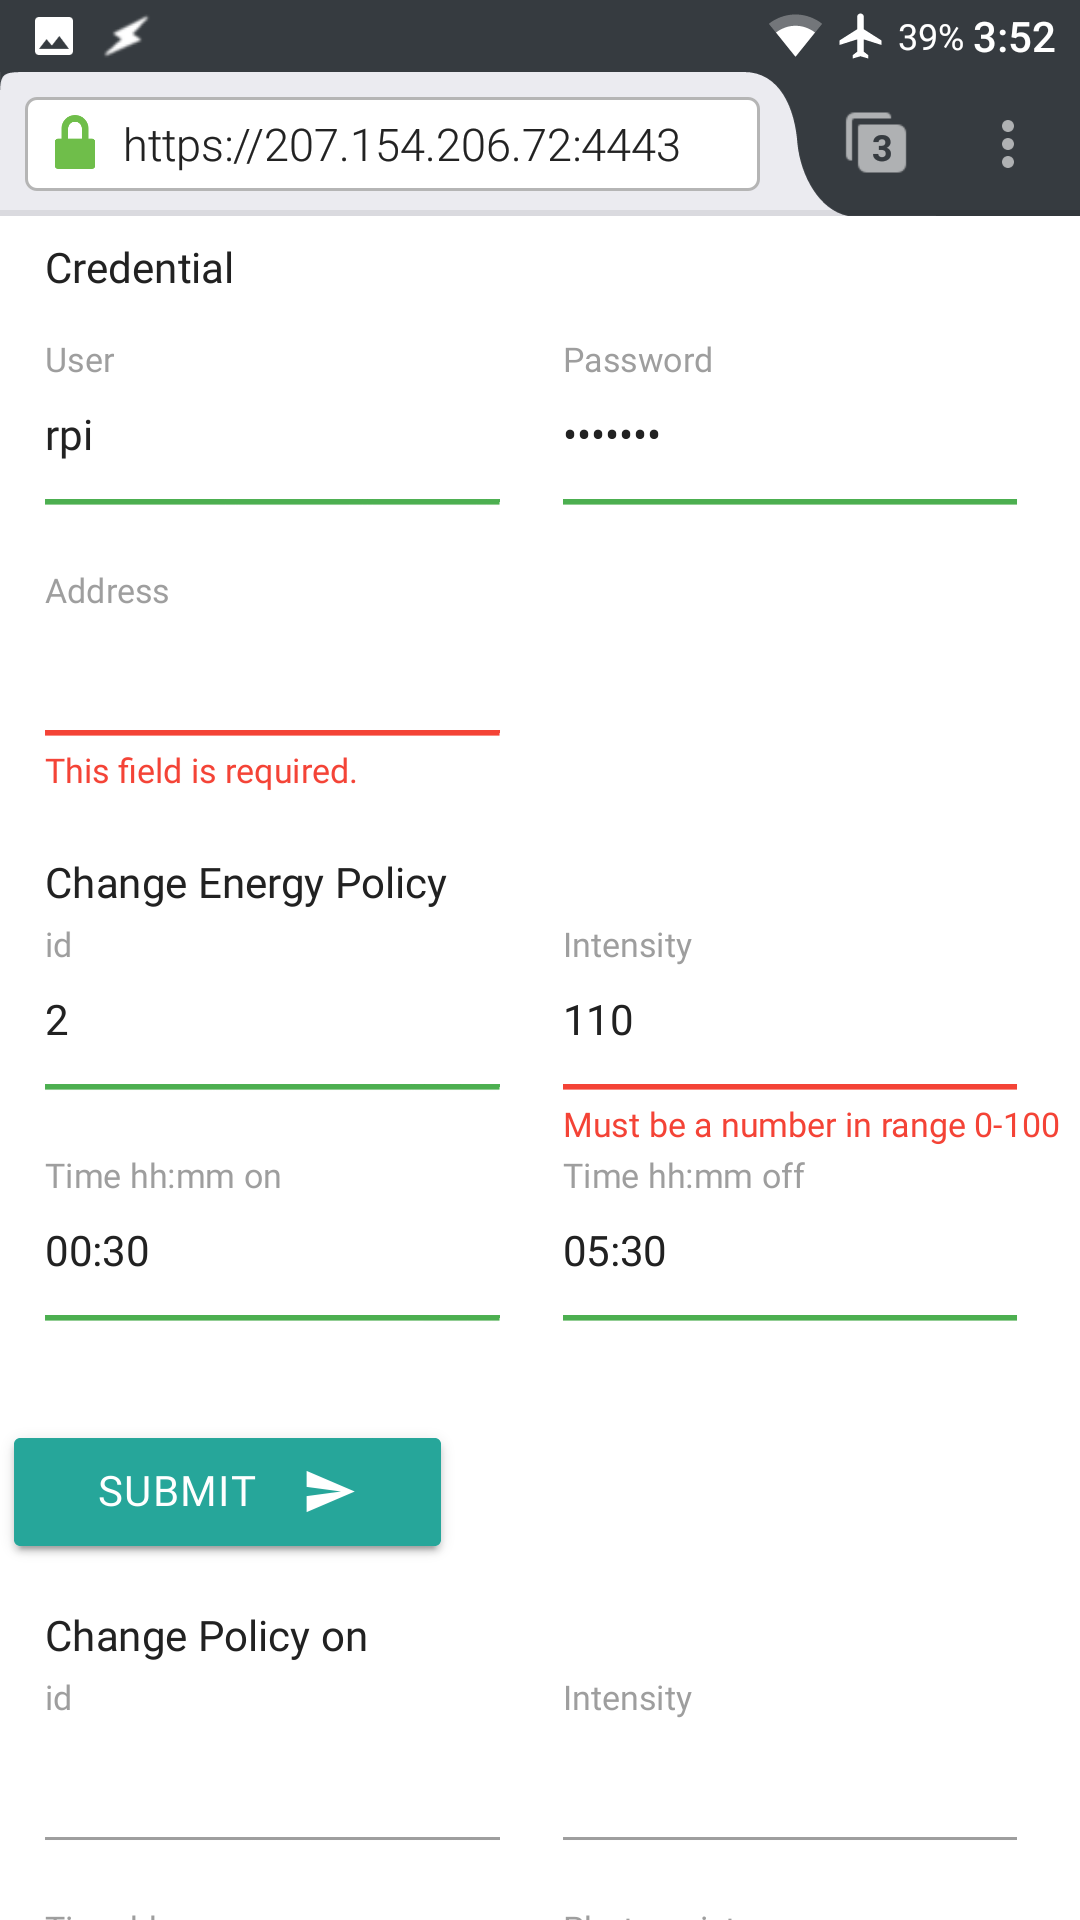
\includegraphics[width=6cm]{figure/web_mobile_errors.png} }}%
	%\caption{Esempi della interfaccia mobile}%
	\label{fig:example}%
\end{figure}

\newpage
\subsection{Linguaggi e librerie}
Nella scelta se realizzare un sito dinamico (con PHP o tecnologie simili) o statico (utilizzando esclusivamente HTML, CSS e Javascript), si è optato per la seconda possibilità, poiché:
\begin{itemize}
 \item il sito consiste in una singola pagina web che contiene sempre le stesse informazioni;
 \item essendo le comunicazioni basate su REST, è il client a contattare direttamente il destinatario, mentre se il sito fosse dinamico, il server fungerebbe da intermediario;
 \item dal punto di vista della sicurezza, evitando di utilizzare PHP si riduce anche la superficie di attacco del server;
 \item essendo il sito piuttosto semplice dal punto di vista delle funzionalità, realizzandolo staticamente è più facile ottenere un design più pulito.
\end{itemize}
Per quanto riguarda lo \textit{style sheet language}, si è valutato di utilizzare direttamente CSS invece di uno strumento di automatizzazione come SASS:
il sito è composto da un'unica pagina Web, di conseguenza uno strumento di come SASS non sarebbe stato di particolare aiuto, e avrebbe inutilmente aggiunto complessità.
Per il CSS si è utilizzata la libreria \textit{materialize}, mentre per quanto riguarda JavaScript sono stati utilizzati \textit{JQuery} e \textit{JQuery validate} (per effettuare controlli client side sui form compilati dagli utenti).


\chapter{Testing}

In questo capitolo veranno descritte le metodologie di test.

\section{Testing della servlet}
Sono stati definiti alcuni test per verificare il funzionamento delle principali parti del programma.

\subsection{Parsing dei parametri}
In questo unit test viene verificata la correttenza della funzione \textit{parseCommandLineParameters}, che esegue il parsing dei parametri specificati tramite command line.
Essendo i parametri scritti dall'utente, è ragionevole pensare che possano essere commessi errori nella digitazione.
Di conseguenza, si è ritenuto utile implementare e verificare il corretto funzionamento di una funzione di questo tipo.

\subsection{Parsing dei messaggi JSON in input}
In questo test viene generata una richiesta HTTP alla servlet, sul modello di quelle provenienti dai Raspberry. Il test verifica che tale richiesta contenga dati JSON sintatticamente e semanticamente corretti.

\subsection{Scrittura di un record sul database}
In questo test viene verificata la corretta comunicazione tra servlet e database, inviando al database una richiesta REST che comporta la scrittura di un record.
Il database invierà l'esito dell'operazione nella risposta. In base al successo o al fallimento dell'operazione, verrà restituito un messaggio di stato HTTP descrittivo.

\subsection{Test di carico}
Poiché i Raspberry sono collegati ad un'istanza della servlet con un rapporto di cardinalità molti a uno, è necessario che la servlet sia in grado di gestire correttamente più richieste contemporaneamente.
In base a quanto affermato in fase di analisi dei requisiti, il caso pessimo è rappresentato da un centinaio o poco più di richieste concorrenti.
Sebbene tale caso pessimo sia molto distante da quello medio, si è valutato di verificare il comportamento della servlet con un carico di quelle dimensioni.
Dai test effettuati, emerge che con l'aumentare delle richieste contemporanee, aumenta il tempo necessario ad elaborarle tutte.
Tuttavia, su una rete a bassa latenza, anche con 150 richieste contemporanee, la servlet non mostra particolari difficoltà, in quanto tutte vengono elaborate prima che vadano in timeout.
Si ritiene che con un tale volume di richieste non si riscontrino particolari problemi anche su reti a media latenza, ma le prestazioni potrebbero essere differenti.
Poiché il tempo necessario per processare una singola richiesta è estremamente ridotto, in realtà la latenza di rete non solo non è particolarmente dannosa, ma in alcuni casi potrebbe anche contribuire ad un bilanciamento del carico nel tempo.
In ogni caso, come precedentemente affermato, si raccomanda di non confidare eccessivamente in una singola istanza della servlet per sistemi di grandi dimensioni, ma di suddividere il carico tra più servlet.


\section{Testing della parte embedded}
Per quanto riguarda gli unit tests della parte Raspberry, si è cercato di ottenere una buona copertura delle funzioni più complesse.
In tutti i test è stato utilizzato il framework \textit{unittest} di Python, inizialmente ispirato a \textit{JUnit} di Java.

\subsubsection{Main Sanity Check \label{msc}}
In questo test si è controllata la correttezza della funzione \textit{sanity\_check} presente nel \textit{main}, richiamata durante la normale esecuzione del programma quando le policy di un lampione vengono modificate, per assicurare che i dati inseriti siano validi.
I controlli che esegue passano dai più intuitivi, come il fatto che l'orario debba essere nell'intervallo numerico 0-23, fino ai più complessi, come la verifica che la fascia oraria di risparmio energetico sia compresa tra l'inizio e la fine delle policy di accensione e spegnimento.
Poiché l'inserimento di fasce orarie include alcuni casi particolari come l'inizio delle policy in un giorno e la fine nel seguente, scrivere un test per validare l'input è di notevole aiuto per prevenire molti errori che potrebbero presentarsi nell'utilizzo reale.
In questo caso potendo essere influente anche il giorno e l'orario in cui si effettua il controllo, si è utilizzata la funzione \textit{patch} offerta da \textit{unittest.mock} per modificare a piacimento il valore relativo alla data corrente.

\subsubsection{Lamp Unit tests}
Sulla classe \textit{lamp} sono stati testati i due metodi statici \textit{get\_delta} e \textit{get\_wait}.
Il metodo \textit{get\_delta} prende come parametri un orario di inizio e uno di fine, e restituisce i secondi di differenza tra i due orari.
Per questo tipo di test si è inserito un orario di inizio uguale alla fine, un orario di fine maggiore di quello di partenza, quindi relativo allo stesso giorno, e con un orario di fine minore, quindi relativo al giorno seguente.
Il metodo \textit{get\_wait}, in modo simile a \textit{get\_delta}, prende come parametri un orario di inizio e uno di fine, e restituisce i secondi di attesa necessari all'inizio dello scheduling.
Se l'orario attuale è già all'interno dello scheduling, verrà restituito un valore negativo corrispondente al numero di secondi già trascorsi dall'inizio.
In questo caso sono stati effettuati diversi test combinando i possibili orari di inizio, fine e l'orario in cui viene effettuata la richiesta.
Per modificare l'orario della richiesta è stata usata la funzione \textit{patch} come nel caso precedente (\ref{msc}).

\subsubsection{Classe RPiMockGPIO}
Per simulare i pin di GPIO del Raspberry Pi è stata creata la classe RPiMockGPIO in modo da simulare l'esecuzione del programma anche senza l'utilizzo fisico di un Raspberry.
Questo si rivela particolarmente utile in fase di design, quando si vuole testare il codice senza avere a disposizione l'hardware.
La funzione di GPIO maggiormente significativa che viene utilizzata nel programma si chiama \textit{wait\_for\_edge} e consiste nell'attesa che un determinato pin cambi stato.
Nel progetto viene utilizzata tutte le volte che si vuole misurare la distanza con il sensore ad ultrasuoni.
Tenendo conto del tempo trascorso tra l'inizio e la fine dell'esecuzione di \textit{wait\_for\_edge} è possibile calcolare la distanza dell'oggetto in prossimità del sensore.
L'implementazione di \textit{wait\_for\_edge} nella classe RPiMockGPIO prevede semplicemente un \textit{time.sleep} su una variabile \textit{wait\_seconds}.
Per questo motivo, regolando il valore di \textit{wait\_seconds} è possibile simulare diversi scenari: impostando un valore alto (come ad esempio 1 secondo) si può simulare una situazione in cui non ci siano mezzi in transito sulle carreggiate;
impostando un valore basso (come 0.001 secondi) si potrà rilevare sempre le auto in transito.

\subsubsection{Schedule test \label{st}}
Questo test permette di controllare la correttezza durante le operazioni di inizializzazione del sistema, di accensione dei lampioni quando si è nella fascia di scheduling, e di successivo spegnimento.
La configurazione del test prevede:
\begin{itemize}
	\item la lettura del file \textit{cfg} di un lampione;
	\item l'impostazione tramite mock object dell'orario corrente a 10 secondi prima dell'inizio dello scheduling;
	\item l'impostazione a 1 secondo della variabile \textit{wait\_seconds}, quindi corrispondente a nessuna auto in transito.
\end{itemize}
A questo punto viene eseguito il \textit{main} del programma e dopo pochi secondi si controlla che il lampione che si sta testando sia spento, in quanto fuori dal suo orario di scheduling.
Avendo impostato inizialmente l'orario corrente a 10 secondi dall'inizio dello scheduling, il sistema aspetta qualche secondo e poi controlla che il lampione sia acceso come da programmazione.
La sua intensità deve corrispondere a quella impostata sul file \textit{cfg}.
Infine si imposta l'ora corrente 1 minuto dopo la fine dello scheduling e si verifica il corretto spegnimento del lampione.

\subsubsection{Test rilevamento auto}
In questo test viene controllata la correttezza durante le operazioni di inizializzazione del sistema, rilevamento di mezzi in transito sulla carreggiata, ritorno a luminosità ridotta quando non sono presenti auto e infine spegnimento alla fine dello scheduling.
La configurazione del test prevede:
\begin{itemize}
	\item la lettura del file \textit{cfg} di un lampione;
	\item l'impostazione tramite mock object dell'orario corrente all'interno della fascia di scheduling di risparmio energetico;
	\item l'impostazione a 0 secondi della variabile \textit{wait\_seconds}, permettendo di rilevare sempre mezzi in transito sulla carreggiata.
\end{itemize}
In seguito viene eseguito il \textit{main} e dopo pochi secondi si verifica che il lampione sia acceso, in quanto il sistema deve avere rilevato automobili sulla carreggiata.
Successivamente si imposta la variabile \textit{wait\_seconds} a 1 secondo, quindi in modo che non vengano più rilevate auto.
Dopo qualche secondo di attesa si controlla che l'intensità del lampione corrisponda al suo valore di risparmio energetico.
Infine, analogamente a quanto avviene per il test della sezione \ref{st}, viene impostata l'ora corrente 1 minuto dopo la fine dello schedule e si controlla che il lampione si sia spento correttamente.


%\chapter*{Ringraziamenti}

%\appendix

\backmatter

%\listoffigures
%\bibliography{biblio}
\bibliographystyle{abbrv}

%\listoftables

\end{document}
